\documentclass[12pt]{article}
\usepackage[T1]{fontenc}
\usepackage[utf8]{inputenc}
\usepackage{graphicx} % includegraphics and all images tools
\usepackage{float}
\usepackage[intlimits]{amsmath}
\usepackage{amssymb,amsfonts}
% \usepackage{txfonts} arial 
\usepackage{fancyhdr} % Extensive control of page headers and footers
\usepackage{fancyvrb}
\usepackage{subcaption}
\usepackage{chngcntr}

\usepackage[hyphens]{url}
\usepackage{hyperref} % links and urls in document
\usepackage{indentfirst} % wcięcie pierwszego akapitu

%begin tick and X emojis
\usepackage{pifont}
\usepackage{xcolor}
\newcommand{\cmark}{\textcolor{green!80!black}{\ding{51}}}
\newcommand{\xmark}{\textcolor{red}{\ding{55}}}
%end

%kolor linków
\hypersetup{
  colorlinks = true, %Colours links instead of ugly boxes
  urlcolor = black, %Colour for external hyperlinks
  linkcolor = black, %Colour of internal links
  citecolor = black %Colour of citations
}

% csharp cmd
\newcommand{\Csharp}{%
  {\settoheight{\dimen0}{C}C\kern-.05em \resizebox{!}{\dimen0}{\raisebox{\depth}{\# }}}}
 %fsharp cmd
\newcommand{\Fsharp}{%
  {\settoheight{\dimen0}{F}F\kern-.05em \resizebox{!}{\dimen0}{\raisebox{\depth}{\# }}}}

% line break after paragraph
\newcommand{\myparagraph}[1]{\paragraph{#1}\mbox{}\\}

\restylefloat{table}
\renewcommand{\contentsname}{Spis treści}
\renewcommand{\abstractname}{}
\renewcommand{\listfigurename}{}
\renewcommand{\listtablename}{}
\let\svaddcontentsline\addcontentsline


\renewcommand{\figurename}{Rys.}
\renewcommand{\tablename}{Tab.}
\renewcommand{\baselinestretch}{1.5}
% \setlength{\textwidth}{14cm}
% \setlength{\textheight}{20cm}
\numberwithin{figure}{section}
\counterwithin{table}{section}

\begin{document}
\begin{sloppypar}
%------------------------------------------------
% Title page
%------------------------------------------------
\begin{titlepage}
 \thispagestyle{empty}
 \begin{center}
  \vspace{3cm}
  \large
    PRACA DYPLOMOWA INŻYNIERSKA\\
  \vspace{4cm}
  \Huge
    Aplikacja dla korepetytorów z płatnościami PayPal w technologii .NET Core\\
  \large
  \vspace{2cm}
  Bartosz Jurczewski, album 210209\\
  \bigbreak
  Politechnika Łódzka\\
  Wydział Fizyki Technicznej, Informatyki i Matematyki Stosowanej\\
  Rok akademicki 2019/2020\\
  \bigbreak
   Promotor: dr hab. inż. Aneta Poniszewska-Marańda \\
   Współpromotor: mgr inż. Krzysztof Stępień\\
 \end{center}
\end{titlepage}

\clearpage
\pagenumbering{arabic}
\setcounter{page}{2}
\setcounter{secnumdepth}{3}
% \setcounter{tocdepth}{4}

%------------------------------------------------
% Main contents
%------------------------------------------------
\tableofcontents
\pagebreak

\pagebreak
%%%%%%%%%%%%%%%%%%%%%%%%%%%%%%%%%%%%%%%%%%%%%%%%%%%%%%%%%%%%
%% Wprowadzenie
%%%%%%%%%%%%%%%%%%%%%%%%%%%%%%%%%%%%%%%%%%%%%%%%%%%%%%%%%%%%
\section{Wprowadzenie}
\textit{Otacza nas rewolucja cyfrowa. Każdy aspekt naszego życia przenosi się do Internetu. Jednym z nich jest rynek usług - korepetycji. Aplikacja internetowa "Find-A-Tutor" jest odpowiedzią na tę rewolucję; pozwala na łatwe zarządzanie korepetycjami - dla ucznia i nauczyciela.}
% Wraz z początkiem lat 70 ubiegłego wieku świat ekonomi nie był już tylko kierowany przez prawa rynku ale także przez otaczający go i postępujący świat cyfryzacji, który z dnia na dzień zmieniał i na nowo definiował działania jego sektorów. 
% Od samego początku cywilizacji Zachodniej, to niewątpliwie ekonomia jej towarzyszyła. 
% Nauką która zawsze towarzyszyła rozwojowi cywilizacji Zachodniej była ekonomia. To właśnie produkcja, konsumpcja czy dystrybucja dóbr napędzała 
% Świat ekonomii wraz z początkiem lat 70 ubiegłego wieku zaczął przechodzić transformacje.
% Wraz z początkiem lat 70 ubiegłego wieku świat ekonomi nie był już tylko kierowany przez prawa rynku
%%%%%%%%%%%%%%%%%%%%%%%%%%%%%%%%%%%%%%%%%%%%%%%%%%%%%%%%%%%%
%% Problematyka
%%%%%%%%%%%%%%%%%%%%%%%%%%%%%%%%%%%%%%%%%%%%%%%%%%%%%%%%%%%%
\subsection{Problematyka} \label{sec:problematyka}
Niewątpliwie czynnikiem, który kształtował ekonomię, rynek lub cywilizację zachodnią jako ogół była zawsze technologia. To ona bezpowrotnie zmieniła oblicze życia w latach 1780–1840 podczas rewolucji przemysłowej i to właśnie ona na nowo definiuje działania naszego świata podczas rewolucji cyfrowej. Początek tej rewolucji datowany jest na lata 70-te XX wieku, ale jej koniec nie został jeszcze wyznaczony, ponieważ przyjmuje się, że trwa ona do dziś.

W 2019 roku prawie 60\% populacji świata miała dostęp do komputera \cite{internet-users}, a w samym 2019 zostało ich sprzedanych prawie 230 tysięcy jednostek \cite{computers}. Obie te liczby przez ostatnie dekady miały tendencję wzrostową, co tylko jeszcze bardziej umacnia obecność technologii w naszym życiu. Niebywałą trudność może sprawić nam znalezienie takiej dziedziny życia, która jeszcze nie została zmodyfikowana przedrostkiem "e" jako jednoznaczny sygnał cyfryzacji.

Pojęcie otaczającego nas wolnego rynku obejmuje również konkurencję. W warunkach idealnych jest to model "konkurencji doskonałej", w którym to każdy z dostawców swoją jakością produktu może rywalizować o pieniądze konsumenta. W dzisiejszych czasach konsument, którego interesuje na przykład wybranie i zakup książki będzie miał do wyboru ponad 10 portali, takich jak \url{www.taniaksiazka.pl}, \url{swiatksiazki.pl}, \url{bonito.pl} lub \url{aros.pl}. Każdy z tych portali oferuje ponad 400 tysięcy pozycji, jak i wiele udogodnieńm, na przykład bezpłatny odbiór w jednej z 125 księgarni w Polsce \cite{ranking}. 

Przyglądając się innym branżom stosującym e-commerce, czyli handel elektroniczny, takim jak: AGD/RTV, artykuły medyczne, zoologiczne, dom i wnętrze, mililitra, motoryzacja, odzież i obuwie, sport, telefony, zdrowie i uroda, zegarki i biżuteria, a nawet żywność, widzimy bogactwo tych rozwiązań wraz z setkami udogodnień dla potencjalnego klienta. 

Obok rynku produktów znajduje się rynek usług. Najczęściej reprezentowany jest przez serwis aukcyjny lub ogłoszeniowy, w którym dany specjalista może zaoferować swój czas i umiejętności za określoną kwotę. Popularnymi i największymi portalami używanymi do tego celu są między innymi \url{olx.pl} lub \url{allegro.pl}.
Ze względu na specyfikę usługi, która nie jest namacalna tak, jak produkt, przedstawienie jej w sposób dokładny może wiązać się z pewnymi trudnościami, przykładowo brak zdjęcia, brak możliwości zmierzenia jej jak produktu lub po prostu mniejsza liczba sposobów na jej opisanie. Sprawia to, że usługi są najczęściej dostępne jako dodatkowa opcja do serwisu handlowego. 

Specyficzną niszą są korepetycje. Oferowane są nie tylko przez nauczycieli akademickich lub nauczycieli innych szkół, ale także przez studentów lub po prostu przez znawców danej dziedziny. Tradycyjnym sposobem znalezienia korepetytora jest szukanie go przez polecenie lub przez papierowe ogłoszenia. Kształt, jak i długość lekcji są najczęściej dostosowywane dopiero przy spotkaniu z daną osobą.

Ostatnim analogowym aspektem korepetycji są oczywiście płatności - dokonywane gotówką. Płatność taka zajmuje zawsze więcej czasu, wiąże się często z wydawaniem reszty i jest nienamierzalna (zależnie od sytuacji jest to zaleta lub wada). Od strony płacącego wiążę się to z brakiem jakiekolwiek historii płatności, a od strony odbiorcy płatności związane jest z jakimkolwiek brakiem historii wpływów, który pozbawia go na przykład możliwości analizowania jego działalności od strony finansowej. 

W tradycyjnym modelu korepetycji to nauczyciel ogłasza się jako osobo świadcząca te usługi. Brakuje jednak rozwiązań, w szczególności w świecie cyfrowym, które pozwoliłby ogłaszać się uczniom jako poszukującym korepetycji. Takie rozwiązanie niewątpliwie powinno łączyć zalety serwisów ogłoszeniowych, odwróconego modelu ogłaszania się (jako ucznia, który tych korepetycji poszukuje) i popularnych płatności on-line. Całość oczywiście powinna być spięta w prosty i intuicyjny interfejs, który swoim minimalizmem nie przytłoczy użytkownika, co często ma miejsce w serwisach powstałych kilka lat temu i zbyt bogatych w treść.
%%%%%%%%%%%%%%%%%%%%%%%%%%%%%%%%%%%%%%%%%%%%%%%%%%%%%%%%%%%%
%% Cel i założenia projektu
%%%%%%%%%%%%%%%%%%%%%%%%%%%%%%%%%%%%%%%%%%%%%%%%%%%%%%%%%%%%
\subsection{Cel i założenia projektu}
Celem niniejszej pracy dyplomowej jest stworzenie aplikacji webowej, która w łatwy sposób pozwoli na zarządzanie korepetycjami ze strony ucznia, jak i ze strony nauczyciela. Aplikacja pozwoli nie tylko na ogłaszanie się i podejmowanie tych ogłoszeń, ale również na płatności internetowe usługą PayPal, jako uniwersalnym rozwiązaniem płatności on-line. 

Stworzony projekt składa się z dwóch warstw: 
aplikacji po stronie serwera (backend) i aplikacji po stronie klienta (frontend).
Frontend został napisany w technologii ASP.NET Razor (generujące dynamiczne strony internetowe po stronie serwera) i fundamentalnych technologiach frontendowych, takich jak HTML, CSS, JavaScript i Bootstrap. Wszelkie dane i operacje są wysyłane do backendu przez protokół HTTP, za pośrednictwem JSONa. 
Backend to RESTful WebApi które zostało napisane w najnowszej obecnie wersji aplikacji szkieletowej .NET Core 2.2.

Funkcje rejestracji i logowania do konta zostały napisane przy wykorzystaniu JWT do uwierzytelnienia użytkownika.

Aby zapewnić bezstanowość API, dane są przechowywane w bazie relacyjnej Microsoft SQL Server.

Dla skalowalności rozwiązania wszystkie usługi zostały zamknięte w kontenerach Docker, bazujących na systemie operacyjnym Linux.

%%%%%%%%%%%%%%%%%%%%%%%%%%%%%%%%%%%%%%%%%%%%%%%%%%%%%%%%%%%%
%% Struktura pracy inżynierskiej
%%%%%%%%%%%%%%%%%%%%%%%%%%%%%%%%%%%%%%%%%%%%%%%%%%%%%%%%%%%%
\subsection{Struktura pracy inżynierskiej}
Pierwszy rozdział pracy jest wstępem do opisanego problemu. Drugi prezentuje ogólną idee ogłoszeń internetowych, skupia się także na płatnościach internetowych oraz opisuje ich bezpieczeństwo. Na końcu przedstawia obecne systemy płatności. Rozdział trzeci pracy skupia się na technicznych aspektach projektu. Opisuje architekturę aplikacji serwerowej (backend) i interfejsu użytkownika (frontend). Czwarty rozdział jest opisem działania stworzonej aplikacji z punktu widzenia użytkownika. 
% \newline
% \newline
% \textit{Rynek usług sprzedawanych za pomocą internetu nie jest rynkiem w całości zagospodarowanym. Ciągle istnieją w niej niższe takie jak rynek korepetycji. Aplikacja Find-A-Turor została przygotowana z myślą o tej niższy.}
%%%%%%%%%%%%%%%%%%%%%%%%%%%%%%%%%%%%%%%%%%%%%%%%%%%%%%%%%%%%
%% Idea ogłoszeń internetowych
%%%%%%%%%%%%%%%%%%%%%%%%%%%%%%%%%%%%%%%%%%%%%%%%%%%%%%%%%%%%
\section{Idea ogłoszeń internetowych}
W czasach przed internetowych, jeśli dana osoba chciała umieścić ogłoszenie lub też przejrzeć listę ogłoszeń miała do wyboru następujące opcje:
\begin{itemize}
    \item gazeta/czasopismo
    \item książka telefoniczna
    \item lokalny bazar (rynek produktów)
    \item ogłoszenie na słupie ogłoszeniowym
    \item opowiedzieć/zapytać o to znajomych
\end{itemize}

Wszystkie opcje mimo swojej prostoty w użytkowaniu, łączyły pewne wady. Podstawową wadą był brak współdzielenia listy ogłoszeń między sobą (np. sekcja ogłoszeń jednej gazety z inną gazetą) lub z innym medium (np. gazeta z czasopismem). Ponad to: brak możliwości wyszukiwania po słowach kluczowych, bezpiecznych płatności na odległość czy też sprawdzenia opinii o danym sprzedawcy.

Po nadejściu rewolucji cyfrowej wszystkie analogowe rozwiązania ogłoszeń zaczęły odchodzić w niepamięć. Należy tutaj wspomnieć o eBayu - największy serwis aukcji internetowych na świecie, który był inspiracją dla autorów - \url{www.allegro.pl} \cite{allegro-wywiad}. Jest to serwis e-commerance (rozszerzony o ogłoszenia i tablice usług), który swoją ofertą dociera do 57,9\% polskich internautów \cite{allegro-liczby}. 

Jednym z największym serwisem ogłoszeniowym na świecie, a największym na rynku indyjskim, brazylijskim i \textbf{polskim} jest serwis \url{www.olx.pl} \cite{olx-wywiad}, który jest częścią grupy OLX Sp. z o.o. W Polsce, w styczniu 2019, olx.pl zanotował 14,4 mln użytkowników, którzy wygenerowali 1,8 miliarda odsłon \cite{olx-liczby}.

Jak pokazują dane rynek ogłoszeń jest bardzo dobrze zagospodarowany i cieszy się ogromną popularnością.
%%%%%%%%%%%%%%%%%%%%%%%%%%%%%%%%%%%%%%%%%%%%%%%%%%%%%%%%%%%%
%% Usługa jako przedmiot ogłoszenia
%%%%%%%%%%%%%%%%%%%%%%%%%%%%%%%%%%%%%%%%%%%%%%%%%%%%%%%%%%%%
\subsection{Usługa jako przedmiot ogłoszenia}
% Obszerny opis jak wygląda ogłoszenie, co tam można napisać, jak się prezentuje produkt a jak usługa
% Korzystając z najpopularniejszego portalu ogłoszeń - olx.pl
Przykładowym portalem który posłuży mi do analizy systemu jest największy serwis ogłoszeniowy w Polsce - \url{www.olx.pl}.

    \begin{figure}[H]
    	\centering
    	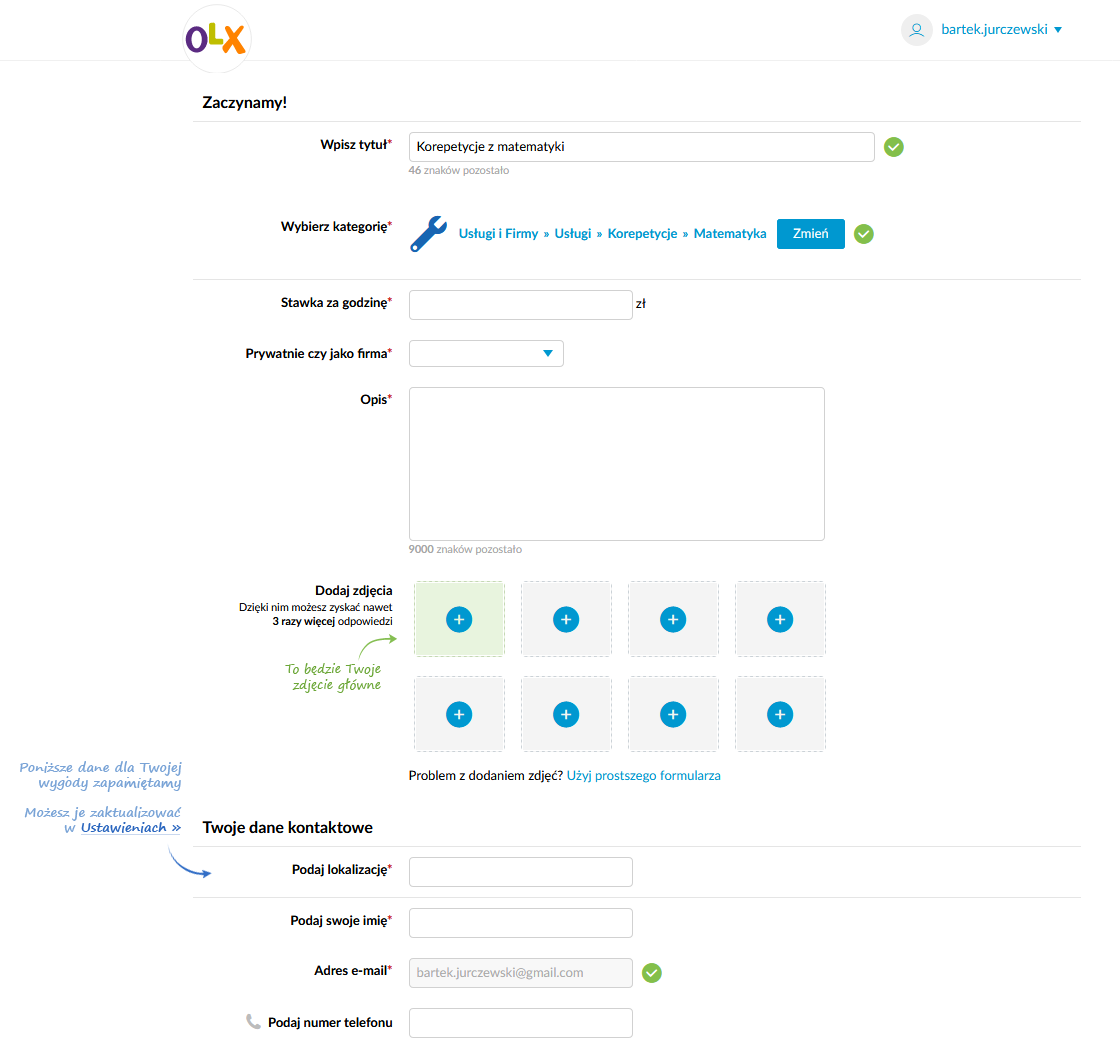
\includegraphics[width=.8\textwidth]{images/chapter_2/olx-add-announcement.png}
    	\caption{Dodawanie ogłoszenia na serwisie OLX}
    	\label{fig:olx-add-announcement}
    \end{figure}

Użytkownik ma do wypełnienia następujące pola:
\begin{itemize}
    \item Tytuł
    \item Kategoria (w tym przypadku Usługi)
    \item Stawka za godzinę
    \item Jakim jest podmiotem gospodarczym
    \item Opis
    \item Dodanie zdjęć
    \item Dane kontaktowe (lokalizacja, imię, nazwisko, adres e-mail, numer telefonu)
\end{itemize}

Jedynym polem które wyróżnia usługę od przedmiotu jest pole "stawka za godzinę". Zgodnie z ideą tego serwisu, użytkownik nie ma możliwości dodania oceny/recenzji po skorzystaniu z jakiejkolwiek usługi, a co za tym idzie porównania ich po ocenach. Dodatkowo serwis ten, całkowicie odrzuca element płatności internetowych (w opozycji do eBaya czy Allegro) i polega wyłącznie na płatności gotówką. Płatności przelewami między użytkownikami są odradzane przez sam OLX, ale są oczywiście możliwe z teoretycznego punktu widzenia. Nie ma jednak wtedy żadnej gwarancji że do takiej wymiany dojdzie, ani możliwości reklamacji czy zwrotu po np. słabo wykonanej usłudze czy otrzymaniu produktu niezgodnego z opisem. Odpowiedzią rynku i rozwoju technologicznego są płatności przez internet.

%%%%%%%%%%%%%%%%%%%%%%%%%%%%%%%%%%%%%%%%%%%%%%%%%%%%%%%%%%%%
%% Płatności internetowe i ich bezpieczeństwo
%%%%%%%%%%%%%%%%%%%%%%%%%%%%%%%%%%%%%%%%%%%%%%%%%%%%%%%%%%%%
\subsection{Płatności internetowe i ich bezpieczeństwo} \label{sec:payments}
Rewolucja cyfrowa dotknęła nie tylko rynku usług i produktów ale także rynku płatności. W samym roku 2016 tylko 16\% kupujących w Polsce opłaciło swoje zakupy gotówką \cite{gotowka}. Liczba rozwiązań płatności internetowych rośnie z każdym rokiem. Aktualnie na rynku jest ich kilka. Każde z nich różni się pod względem komfortu użytkowania, szybkości jak i bezpieczeństwa. 

%%%%%%%%%%%%%%%%%%%%%%%%%%%%%%%%%%%%%%%%%%%%%%%%%%%%%%%%%%%%
%% Zwykły przelew bankowy
%%%%%%%%%%%%%%%%%%%%%%%%%%%%%%%%%%%%%%%%%%%%%%%%%%%%%%%%%%%%
\subsubsection{Zwykły przelew bankowy}
Jest to najprostsze i najbardziej analogowe rozwiązanie. Zaraz po złożeniu zamówienia, dostajemy potwierdzenie mailem wraz z numerem konta sprzedawcy, kwoty zamówienia i tytułem przelewu (który najczęściej jest numerem zamówienia). Na kupującym ciąży zalogowanie się na stronę banku, utworzenie nowego przelewu i co istotne wypełnienie ich danymi. Oprócz możliwości pomyłki np. przekopiujemy nie pełny numer zamówienia pomijając jeden znak, ryzykiem o którym musimy pamiętać jest obecność złośliwego oprogramowania. Przykładem może być głośna sprawa z roku 2018, w którym to firma ESET natrafiła na konia trojańskiego - BackSwap. Portal \url{www.zaufanatrzeciastrona.pl} opisuje go następująco: "Do wstrzyknięcia dochodzi w momencie, gdy klient zleca przelew. Złośliwy kod podmienia wtedy numer rachunku, na który ma zostać wysłany przelew ofiary. Na ekranie komputera tego nie widać – zmiana dotyczy informacji, które przeglądarka wysyła do banku. Przestępcy nie atakują wszystkich przelewów – definiują konkretny przedział kwotowy, który ich interesuje. Ostatnio celowali w kwoty między 10 000 a 20 000 PLN."\cite{backswap}.
Takie ataki są niestety ciągle spotykane. Niektóre banki jak np. ING Bank Śląski, po skopiowaniu numeru rachunku bankowego usuwa dwie pierwsze cyfry i prosi klienta o uzupełnienie ich. Bank próbuje wymusić podwójne sprawdzenie numeru konta. Efektem ubocznym będzie możliwość pomyłki przy ponownym wprowadzaniu go.

Szybkość takiego rozwiązania jest zależna od godziny wysłania przelewu. Jest to spowodowane godzinami sesji rozliczeniowych w danych bankach. Najczęściej jeśli przelew zostanie wysłany do południa, dotrze on pod wieczór. W przypadku późniejszych przelewów, dojdzie on kolejnego dnia roboczego. Wszystkie przelewy w święta i weekendy również dochodzą dopiero kolejnego dnia roboczego. Taka płatność opóźnia wysyłkę/realizację usługi, ponieważ zostanie ona wykonana dopiero wtedy gdy na rachunku pojawią się przelane środki. 

%%%%%%%%%%%%%%%%%%%%%%%%%%%%%%%%%%%%%%%%%%%%%%%%%%%%%%%%%%%%
%% Przelewy pay-by-link
%%%%%%%%%%%%%%%%%%%%%%%%%%%%%%%%%%%%%%%%%%%%%%%%%%%%%%%%%%%%
\subsubsection{Przelewy pay-by-link}
Ta forma płatności cieszy się największą popularnością w Polsce \cite{jak-placa-polacy}. Po wykonaniu zakupów, wybieramy opcję przelewu online, następnie z listy banków, pokazanych na rysunku \ref{fig:pay-by-link} wybieramy ten z którego chcemy dokonać płatności. 

\begin{figure}[H] 
 	\centering
	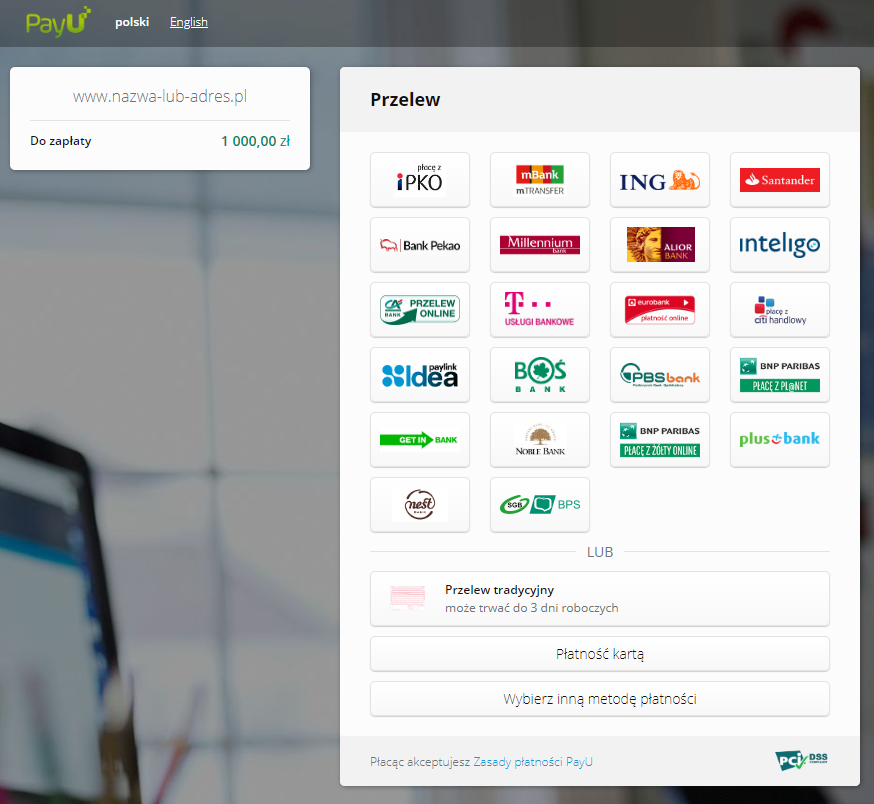
\includegraphics[width=1\textwidth]{images/chapter_2/pay-by-link.png}
	\caption{Przykładowa płatność pay-by-link}
	\label{fig:pay-by-link}
\end{figure}

Po kliknięciu zostajemy przeniesieni na stronę logowania do danego banku. Po wpisaniu loginu i hasła, pojawi się uzupełniony szablon przelewu który kupujący musi tylko zatwierdzić. Ostatnim krokiem, kluczowym od strony bezpieczeństwa jest SMS z kodem autoryzacyjnym który otrzymamy. Klient musi przepisać owy kod aby potwierdzić przelew. Dzięki temu nawet, jeśli ktoś poznał nasze dane logowania, nie będzie ich mógł użyć do płatności bez posiadania naszego telefonu. Alternatywnym i co raz bardziej popularnym rozwiązaniem jest potwierdzenie przelewu przez aplikację banku. Za nim jednak będzie to możliwe, użytkownik musi się do niej zalogować, co oznacza dodatkowy etap bezpieczeństwa.

Po poprawnym uwierzytelnieniu i potwierdzeniu transakcji, środki trafią niemal natychmiast do sprzedawcy, dzięki czemu od razu będzie wstanie zrealizować zamówienie.

%%%%%%%%%%%%%%%%%%%%%%%%%%%%%%%%%%%%%%%%%%%%%%%%%%%%%%%%%%%%
%% Karta płatnicza
%%%%%%%%%%%%%%%%%%%%%%%%%%%%%%%%%%%%%%%%%%%%%%%%%%%%%%%%%%%%
\subsubsection{Karta płatnicza} \label{sec:cards}
W maju 1898 firma Sequoia Data Corp. wprowadziła na rynek Compumarket, pierwszy internetowy system e-commerce obsługujący płatności kartą kredytową. Od tego czasu płatności kartą zyskały wiele nowych usprawnień jednak ich rdzeń pozostał nietknięty. Aby zrealizować płatność, kupujący jest proszony o wpisanie trzech danych: numeru karty, daty jej ważności oraz trzycyfrowego kodu CVC/CVV znajdującego się na odwrocie karty. Po ich zweryfikowaniu, płatność zostaje zakończona. Ta metoda jest tak samo szybka jak pay-by-link ale mniej wygodna, ponieważ za każdym razem musimy ponownie wpisać dane karty. 

Tradycyjny model zakładał nasze zaufanie do portalu w którym dokonujemy zakupów, ponieważ osoba posiadająca owe dany karty mogła samodzielnie dokonać płatności bez naszej zgody. Odpowiedzią na to jest coraz częściej obecna usługa bankowa 3D Secure. Polega ona na dodatkowym etapie weryfikacji. Po poprawnym wpisaniu danych karty i ich zweryfikowaniu, klient otrzymuje SMSa z kodem weryfikacyjnym. Dopiero po wprowadzeniu go, transakcja jest finalizowana.

Zaletą która wyróżnia ten rodzaj płatności jest usługa chargeback. Portal \url{www.najlepszekonto.pl} opisuje ją następująco: "Chargeback, czyli obciążenie zwrotne, to usługa dostępna tylko dla kart płatniczych. Polega ona na zwrocie środków z konta sprzedawcy, jeśli kupiony przez Ciebie towar nie spełnił Twoich oczekiwań: miał wady, różnił się od tego, co obiecywał sprzedawca, lub w ogóle go nie otrzymałeś. Jeśli próby wymiany towaru w sklepie nie powiodą się, możesz zwrócić się z prośbą o rozstrzygnięcie sprawy przez bank, który jest wystawcą Twojej karty."\cite{chargeback}.

Odmianą fizycznej karty płatniczej jest karta wirtualna. Taka karta usłuży tylko do płatności internetowych. Nie użyjemy jej np. podczas zakupów w sklepie. Po jej wyrobieniu, bank nie przesyła nam jej pocztą, a po prostu podaje nam ich dane (numer, data ważności i kod CVC/CVV). Niewątpliwą zaletą jest bezpieczeństwo - nie padniemy ofiarą skimmingu (nielegalne skopiowanie zawartości paska magnetycznego w celu utworzenia kopii). Główną wadą takie rozwiązania jest dostępność w Polsce. Aktualnie tylko dwa banki udostępniają taką usługę - i to za miesięczną opłatą. 

Zagranicznymi serwisami które utworzenie wirtualnych kart, jest np. amerykański \url{www.privacy.com}. Portal ten pozwala na proste i nielimitowane tworzenie kart wirtualnych, jak możemy przeczytać na stronie firmy, "jednym kliknięciem". Klient ma możliwość tworzenia karty per portal (np. jedna karta do Netflixa, kolejna do opłacenia Spotify), dodatkowo może ustawić limit obciążenia dla danej strony, wstrzymać płatność lub całkowicie zablokować niechciane opłaty. 

%%%%%%%%%%%%%%%%%%%%%%%%%%%%%%%%%%%%%%%%%%%%%%%%%%%%%%%%%%%%
%% Portfele elektroniczne
%%%%%%%%%%%%%%%%%%%%%%%%%%%%%%%%%%%%%%%%%%%%%%%%%%%%%%%%%%%%
\subsubsection{Portfele elektroniczne}

Hybrydą wymienionych wcześniej rozwiązań są portfele elektroniczne zwane również portfelami cyfrowymi. Rozwiązanie te charakteryzuje się następującymi funkcjonalnościami: 
portfel wirtualny (rozumiany jako pula środków do wykorzystania) wraz z możliwością przelania ich bezpośrednio na rachunek bankowy, płatność wieloma podpiętymi kartami (kredytowymi jak i debetowymi), także w innych walutach, możliwość określenia adresu dostawy klienta i innych informacji ułatwiających sfinalizowanie zamówienia. Kolejnym udogodnieniem jest przechowywanie środków w różnych walutach, dzięki czemu użytkownik nie jest obciążony podwójnym przewalutowaniem.

Niektóre portfele oferują też świadczenie usług bez jakikolwiek przelanych środków i potrafią służyć jako zaufany pośrednik płatności. Jeśli tylko mamy podpiętą kartę/karty pod taki portfel, możemy w dowolnym miejscu zapłacić owym portfelem, a należność zostanie ściągniętą natychmiast z naszej wybranej karty. Dzięki czemu nie jesteśmy wystawieni na potencjalne wady używania samej karty jako środka płatności opisanych w rozdziale \ref{sec:cards}.

%%%%%%%%%%%%%%%%%%%%%%%%%%%%%%%%%%%%%%%%%%%%%%%%%%%%%%%%%%%%
%% Obecne rozwiązania
%%%%%%%%%%%%%%%%%%%%%%%%%%%%%%%%%%%%%%%%%%%%%%%%%%%%%%%%%%%%
\subsection{Obecne rozwiązania}
Przez lata rozwiązania na rynku usług jak i płatności ewoluowały. Często stając się osobnym bytem, a nie dodatkiem jak na początku ich istnienia. Firmy odpowiedzialne za nie, przez lata starały się udoskonalić swój produkt i jak najlepiej go wypromować. Poniższe zestawienie zostało podzielone na dwie grupy: płatności (jako rdzeń serwisu usług) i serwisy dla korepetytorów.

%%%%%%%%%%%%%%%%%%%%%%%%%%%%%%%%%%%%%%%%%%%%%%%%%%%%%%%%%%%%
%% Płatności
%%%%%%%%%%%%%%%%%%%%%%%%%%%%%%%%%%%%%%%%%%%%%%%%%%%%%%%%%%%%
\subsubsection{Płatności}
Szukając odpowiedniego rozwiązania do obsługi płatności, autor miał na celu trzy główne cechy: szybkość (jak szybko środki trafią na konto), wygodę (a w tym szybkość wykonania samej płatności) i bezpieczeństwo (transakcji jak i procesów około transakcyjnych). Każde z czterech dostępnych rozwiązań zostało szczegółowo opisane w rozdziale \ref{sec:payments}, właśnie pod kątem tych trzech cech. Stosując takie kryterium, autor uznaje portfel elektroniczny jako zwycięzce w tych trzech kategoriach. Dlatego w dalszym rozważaniu obecnych rozwiązań będzie brał tylko je pod uwagę.

\begin{table}[H]
    \begin{tabular}{|p{5cm}|c|c|c|}
    \hline
     & \multicolumn{1}{l|}{\textbf{PayPal}} & \multicolumn{1}{l|}{\textbf{Visa Checkout}} & \multicolumn{1}{l|}{\textbf{Masterpass}} \\ \hline
    Język polski & \cmark & \cmark & \cmark \\ \hline
    Podpięcie adresu dostawy & \cmark & \cmark & \cmark \\ \hline
    Uwierzytelnianie mailem & \cmark & \cmark & \xmark \\ \hline
    Używanie kart różnych firm & \cmark & \xmark & \xmark \\ \hline
    Możliwość dwustopniowego uwierzytelniania & \cmark & \xmark & \cmark \\ \hline
    Możliwość przechowywania środków w portfelu & \cmark & \xmark & \xmark \\ \hline
    \end{tabular}
    \caption{Porównanie portfeli elektronicznych}
    \label{tab:portfele}
\end{table}

Zestawienie pokazane w tabeli \ref{tab:portfele} pokazuje, że PayPal wygrywa w dwóch funkcjonalnościach z Visa Checkout i Masterpassem: użycie kart różnych firm i możliwość przechowywania środków w portfelu.

Ponadto, VisaCheckout i Masterpass są realizowane jako zamknięte środowiska płatnicze. Po kliknięciu na przycisk oznaczony ich logiem, zostajemy przeniesieni do realizacji płatności. PayPal zdecydował się na inne rozwiązanie. Ich rozwiązanie daje klientowi możliwość zapłaty kartą (Visa, MasterCard i Amex), polskim portalem Przelewy24 (który agreguje płatności pay-by-link i kartą - omówione w rozdziale \ref{sec:payments}) i portfelem cyfrowym PayPal. 

\begin{figure}[H] 
 	\centering
	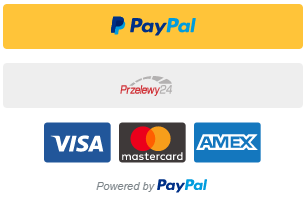
\includegraphics[scale=1.0]{images/chapter_2/paypal-button.png}
	\caption{Smart Payment Button}
	\label{fig:paypal-button}
\end{figure}

PayPal określa swój przycisk jako \textbf{Smart Payment Button} (ang. 
inteligentny przycisk do płatności), przedstawiony na rysunku \ref{fig:paypal-button}. Oprócz łączenia kilku sposobów płatności, może różnić się on w każdym kraju. Np. w Polsce wspiera on portal Przelewy24. Dzięki elastyczności \textit{smart payment button} możemy być pewni że zostanie on dostosowany do kraju z którego zostaje dokonywane zamówienie, co potencjalnie może zwiększyć zyski ze względu na bogactwo opcji płatności. 

Podsumowując, w grupie portfeli elektronicznych, rozwiązanie PayPal wspiera wszystkie kluczowe i istotne dla mnie funkcjonalności. Dlatego też, to ono zostanie zaimplementowane w aplikacji \textit{Find-A-Tutor} w celu wspierania płatności on-line.

%%%%%%%%%%%%%%%%%%%%%%%%%%%%%%%%%%%%%%%%%%%%%%%%%%%%%%%%%%%%
%% Serwisy dla korepetytorów
%%%%%%%%%%%%%%%%%%%%%%%%%%%%%%%%%%%%%%%%%%%%%%%%%%%%%%%%%%%%
\subsubsection{Serwisy dla korepetytorów}
Na rynku polskim są obecnie trzy największe serwisy dla korepetytorów. Są to www.e-korepetycje.net, 
korepetycje.net i wspomniany już wcześniej portal, nie tylko do korepetycji - olx.pl. Poniżej zestawiono ze sobą cechy tych portali. Cechy zostały zaczerpnięte z rozdziału \ref{sec:problematyka} pokrywającego problematykę pracy.

\begin{table}[H]
    \begin{tabular}{|p{5cm}|c|c|c|c|}
    \hline
     & \multicolumn{1}{l|}{e-korepetycje.net} & \multicolumn{1}{l|}{korepetycje.net} & \multicolumn{1}{l|}{olx.pl} \\ \hline
    Możliwość płatności online & \xmark & \xmark & \xmark \\ \hline
    Ogłoszenia dodawane przez uczniów & \cmark & \xmark & \cmark \\ \hline
    Minimalistyczny design & \cmark & \xmark & \xmark \\ \hline
    Otwarte API & \xmark & \xmark & \xmark \\ \hline
    Aplikacja mobilna & \xmark & \xmark & \cmark \\ \hline
    \end{tabular}
    \caption{Porównanie serwisów dla korepetytorów}
    \label{tab:korepetycje}
\end{table}

Żaden z portali zestawionych powyżej nie obsługuje funkcjonalności tak podstawowej w dzisiejszym świecie jak płatności elektroniczne. Tylko jeden z nich oferuje przyjazny dla oka i wpisujący się w obecne trendy - minimalisty design. Dodatkowo e-korepetycje.net i korepetycje.net nie posiadają otwartego API, które może posłużyć do stworzenia w przyszłości aplikacji mobilnych. Jednym portalem który ją dostarcza, jest OLX.pl.
\newline
\newline
\textit{Obserwując rynek korepetycji, brakuje na nim rozwiązania które wspiera płatności online. Taką aplikacją jest Find-A-Tutor. Dodatkowo, backend został stworzony jako otwarte API, dzięki czemu w przyszłości serwis będzie otwarty na powstanie aplikacji mobilnych. Fundamentalną funkcjonalnością będzie dodawanie ogłoszeń przez studentów. Całość została spięta minimalistycznym i nieprzytłaczającym designem.}

%%%%%%%%%%%%%%%%%%%%%%%%%%%%%%%%%%%%%%%%%%%%%%%%%%%%%%%%%%%%
%% Techniczne aspekty aplikacji Find-A-Tutor
%%%%%%%%%%%%%%%%%%%%%%%%%%%%%%%%%%%%%%%%%%%%%%%%%%%%%%%%%%%%
\section{Techniczne aspekty aplikacji \textit{Find-A-Tutor}} \label{tech-aspect}

%%%%%%%%%%%%%%%%%%%%%%%%%%%%%%%%%%%%%%%%%%%%%%%%%%%%%%%%%%%%
%% Wymagania
%%%%%%%%%%%%%%%%%%%%%%%%%%%%%%%%%%%%%%%%%%%%%%%%%%%%%%%%%%%%
\subsection{Wymagania}
W tym rozdziale autor opisuje wymagania aplikacji webowej \textit{Find-A-Tutor}, dzieląc je na funkcjonalne i niefunkcjonalne. 

%%%%%%%%%%%%%%%%%%%%%%%%%%%%%%%%%%%%%%%%%%%%%%%%%%%%%%%%%%%%
%% Wymagania funkcjonalne
%%%%%%%%%%%%%%%%%%%%%%%%%%%%%%%%%%%%%%%%%%%%%%%%%%%%%%%%%%%%
\subsubsection{Wymagania funkcjonalne}
Wymagania funkcjonalne to spisane zasady, jak aplikacja ma się zachować po wystąpieniu danego zdarzenia/zapytania. Wymagania te jasno określają funkcje jakie ma mieć aplikacja, problemów jakie ma ona rozwiązywać, a także opisują jej ogólną wizję \cite{funkcjonalne}. \\
\noindent
\textbf{Rejestracja jako uczeń lub korepetytor}\\
\indent
Formularz rejestracji pozwala na rejestrację jako użytkownik z wyróżnieniem ucznia i użytkownika. Oba ta konta moją inne uprawnienia i funkcjonalności opisane poniżej.

\noindent
\textbf{Logowanie jako uczeń, korepetytor i administrator}\\
\indent  
Dostępny panel logowania dla użytkownika (ucznia lub korepetytora). Dodatkowym rodzajem konta jest administrator, który ma pełne uprawnienia do działania na systemie. Takie konto nie posiada panelu użytkownika, ale może dokonywać wszelakich operacji opisanych w osobnym punkcie, używając zapytań do API.

\noindent
\textbf{Panel ucznia}\\
\indent
Panel dostępny dla użytkownika zalogowanego jako student. Umożliwia podgląd wszystkich ogłoszeń zgłoszonych przez danego ucznia. Dodatkowo powinien on wyświetlać podstawowe dane takie jak: data utworzenia, datę podjęcia ogłoszenia, opis, datę wygaśnięcia ogłoszenia, przedmiot, status płatności i status ogłoszenia. Logowanie następuje przez przeglądarkę internetową. 

\noindent
\textbf{Podgląd szczegółów ogłoszenia}\\
\indent
Uczeń powinien mieć dostęp do widoku szczegółowego ogłoszenia, który pokazuje wszystkie informacje na temat ogłoszenia.

\noindent
\textbf{Dodawanie ogłoszeń}\\
\indent
Możliwość dodania ogłoszenia przez użytkownika - ucznia. Użytkownik uzupełnia następujące dane: opis, data przedawnienia ogłoszenia, przedmiot (wybrany z listy przedmiotów). 

\noindent
\textbf{Płatności online za lekcje}\\
\indent
Po przypisaniu ogłoszenia do korepetytora, student ma możliwość opłacenia należności za ogłoszenie online. Po opłaceniu, ma to odzwierciedlenie w statusie. 

\noindent
\textbf{Finalizacja ogłoszenia}\\
\indent
Po odbytej lekcji, użytkownik zaznacza zakończenie takiej lekcji, tym samej zmieniając jej status.

\noindent
\textbf{Panel korepetytora}\\
\indent
Użytkownik korepetytor, po zalogowaniu ma dostęp do swojego panelu ze wszystkimi dostępnymi ogłoszeniami i ze wszystkimi podjętymi przez niego ogłoszeniami. Dostępne są na nim następujące informacje: data utworzenia, datę podjęcia ogłoszenia, opis, datę wygaśnięcia ogłoszenia, przedmiot, status płatności i status ogłoszenia. Logowanie następuje przez przeglądarkę internetową. 
\clearpage
\noindent
\textbf{Podjęcie ogłoszenia}\\
\indent
Korepetytor ma możliwość podjęcie ogłoszenia z puli nieprzydzielonych ogłoszeń. Podaje on swoją stawkę godzinową wyrażoną w złotówkach. Stawka ta zostaje przypisana do ogłoszenia wraz z kwotą należną za całe ogłoszenie (stawka pomnożona przez liczbę godzin). Po operacji podjęcia, zmienia on swój status.

\noindent
\textbf{Oddanie ogłoszenia}\\
\indent
Jeśli ogłoszenie, po podjęciu, nie zostało jeszcze opłacone, korepetytor ma możliwość zwrócenia ogłoszenia do ogólnej puli ogłoszeń., tym samym jego status wraca do stanu wejściowego. 

\noindent
\textbf{Konto administratora}\\
\indent
Po zalogowaniu się zapytanie, taki użytkownik może wykonywać operacje CRUD (ang. create, read, update and delete (pol. utwórz, odczytaj, aktualizuj i usuń)) na ogłoszeniach, użytkownikach i przedmiotach. Dodatkowo ma możliwość wszystkich operacji ucznia czy korepetytora.

%%%%%%%%%%%%%%%%%%%%%%%%%%%%%%%%%%%%%%%%%%%%%%%%%%%%%%%%%%%%
%% Wymagania niefunkcjonalne
%%%%%%%%%%%%%%%%%%%%%%%%%%%%%%%%%%%%%%%%%%%%%%%%%%%%%%%%%%%% 
\subsubsection{Wymagania niefunkcjonalne}

Wymagania niefunkcjonalne określają obszar jakości aplikacji. Wynikają często z wymagań funkcjonalnych lub architektonicznych. Źródłem tych wymagań są przyszli użytkownicy oraz klienci. Są to np. skalowalność, kompatybilność czy bezpieczeństwo \cite{niefunkcjonalne}.\\
\noindent
\textbf{Przenośność}\\
\indent
Aplikacja powinna być łatwa w zmianie lokalizacji, środowiska, eksportu danych.

\clearpage
\noindent
\textbf{Skalowalność}\\
\indent
Aplikacja powinna móc się skalowalność pionowo (zwiększenie mocy serwera) i poziomo (zwiększenie instancji aplikacji).

\noindent
\textbf{Otwartość na rozszerzenia}\\
\indent
Aplikacja powinna mieć otwarte API (backend) i być gotowa na nowe urządzenia które mogą z niej korzystać (np. mobilne).

\noindent
\textbf{Kompatybilność}\\
\indent
Aplikacja powinna działać w technologiach uniwersalnych i powszechnych dla przeglądarkę na silniku Chromium (Chrome, Opera i wkrótce Edge), który na rynku polskim ma 80,65\% podziału rynku \cite{chrome}.

\noindent
\textbf{Bezpieczeństwo}\\
\indent
Dane użytkowników powinny być poufne i dostępne dla danego użytkownika po zalogowaniu.

\noindent
\textbf{Użyteczność }\\
\indent
Aplikacja powinna być łatwa w obsłudze i powinna być okraszona minimalistycznym designem który nie przytłacza użytkownika.

\noindent
\textbf{Modularność}\\
Warstwa bazy danych, graficzna i aplikacji (API) powinny być od siebie oddzielone i gotowe do zastąpienia.
    
%%%%%%%%%%%%%%%%%%%%%%%%%%%%%%%%%%%%%%%%%%%%%%%%%%%%%%%%%%%%
%% Narzędzia i technologie użyte w projekcie
%%%%%%%%%%%%%%%%%%%%%%%%%%%%%%%%%%%%%%%%%%%%%%%%%%%%%%%%%%%% 
\subsection{Narzędzia i technologie użyte w projekcie}
Podczas realizacji aplikacji zostały wybrane tylko te technologie i rozwiązania, które wyrobiły mocną pozycję w świecie inżynierii oprogramowania. Są to narzędzia dostępne od lat, sprawdzone w wielu aplikacjach i zalecane w projektach webowych. Dodatkowo za cel przyjął sobie takie pojęcia jak czysty kod, czysta architektura oraz korzystanie z jak największej liczby gotowych rozwiązań - tak aby nie rozwiązywać po raz kolejny tych samych problemów.

%%%%%%%%%%%%%%%%%%%%%%%%%%%%%%%%%%%%%%%%%%%%%%%%%%%%%%%%%%%%
%% .NET Core 2.2
%%%%%%%%%%%%%%%%%%%%%%%%%%%%%%%%%%%%%%%%%%%%%%%%%%%%%%%%%%%%    
\subsubsection{.NET Core 2.2}
.NET Core jest darmowym i otwartym frameworkiem dla systemów Windows, Linux i macOS. Jest wielo-platformowym następcą .NET Framework. Projekt jest rozwijany przez Microsoft i dystrybuowany na zasadach otwartego oprogramowania (ang. open source). Składa się z on narzędzi programistycznych, bibliotek oraz środowiska uruchomieniowego \cite{dotnet-core}. 
    
Charakteryzują go następujące cechy:
\begin{itemize}
    \item Możliwość programowania i uruchamiania w systemach Windows,\\ macOS i Linux,
    \item Zunifikowany scenariusz tworzenia interfejsu API sieci Web i internetowych sieci Web,
    \item System konfiguracji oparty na środowisku, który jest gotowy do chmury,
    \item Wbudowane wstrzykiwanie zależności,
    \item Lekki, wysoko wydajny modularny potok żądań HTTP,
    \item Otwarte i skoncentrowane na społeczności,
    \item Obsługa wielu języków programowania: \Csharp, \Fsharp i także Visual Basic,
    \item Obsługa menadżera pakietów NuGet,
    \item Elastyczny w wdrożeniu, np. kontereryzacja za pomocą Dockera
\end{itemize}
%%%%%%%%%%%%%%%%%%%%%%%%%%%%%%%%%%%%%%%%%%%%%%%%%%%%%%%%%%%%
%% C#
%%%%%%%%%%%%%%%%%%%%%%%%%%%%%%%%%%%%%%%%%%%%%%%%%%%%%%%%%%%% 
\subsubsection{C\#}
\Csharp (ang. C sharp) jest językiem obiektowym, opracowanym dla firmy Microsoftu, na przełomie tysiąclecia przez zespół pod kierownictwem Andersa Hejlsberga. Jak możemy przeczytać w oficjalnej dokumentacji Microsoftu: 
"Programiści znający którykolwiek z tych języków (C, C++, Java) są zazwyczaj w stanie zacząć produktywnie pracować w \Csharp w bardzo krótkim czasie. Składnia w języku \Csharp upraszcza wiele złożoności C++ i zapewnia zaawansowane funkcje, takie jak typy dopuszczające wartości zerowe, wyliczenia, delegaty, wyrażenia lambda i bezpośredni dostęp do pamięci, których nie można znaleźć w Javie." \cite{csharp} 
    
Podczas opracowywania go, zespołowi przyświecały poniższe cele:
\begin{itemize}
    \item obiektowość,
    \item prostota i nowoczesność,
    \item wsparcie dla istniejących zasad Inżynierii Oprogramowania, takich jak:
    \begin{itemize}
       \item silne typy,
       \item automatyczne czyszczenie śmieci z pamięci (ang. garbage collector),
       \item wykrywanie każdej próby odniesienia się do niezainicjowanych zmiennych
    \end{itemize}
\end{itemize}
    
Jako język obiektowy \Csharp obsługuje pojęcia enkapsulacji, dziedziczenia i polimorfizmu. Wszystkie zmienne i metody, w tym metoda Main, punkt wejścia aplikacji, są zawarte w definicjach klas. Klasa może dziedziczyć bezpośrednio od jednej klasy nadrzędnej, ale może implementować dowolną liczbę interfejsów.

% \subsubsection{Docker}

%%%%%%%%%%%%%%%%%%%%%%%%%%%%%%%%%%%%%%%%%%%%%%%%%%%%%%%%%%%%
%% Kontrola dostępności serwisu
%%%%%%%%%%%%%%%%%%%%%%%%%%%%%%%%%%%%%%%%%%%%%%%%%%%%%%%%%%%% 
\subsubsection{Kontrola dostępności serwisu}
Celem kontroli stanu projektu jest uzyskanie niezależnej oceny, w dowolnym momencie cyklu życia projektu, tego jak dobrze program działa, czy działa zgodnie z jego celami i jak dobrze przestrzega najlepszej metodologii praktyki. Skuteczna kontrola stanu (ang. health check) zapewni dostęp do informacji o stanie zależności owego projektu np. czy program ma połączenie z bazą lub pokaże w jakiej "kondycji" jest nasz program np. jaki czas zajmuje mu połączenie i wywołanie prostego zapytania na bazie. 
    
Rozwiązaniem które dostarcza kontrole stanów prawie trzydziestu różnych komponentów jest \textbf{AspNetCore.Diagnostics.HealthChecks} \cite{health-checks-github}.
        
\begin{figure}[H] 
    \centering
    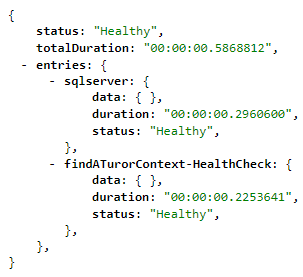
\includegraphics[width=0.5\textwidth]{images/chapter_3/api-health-check.png}
    \caption{Kontrola kondycji aplikacji \textit{Find-A-Tutor}}
    \label{fig:health-check}
\end{figure}
    
Rysunek \ref{fig:health-check} pokazuje stan zależności projektu (backend), wraz z dostępem do bazy danych i czasem który potrzebował na wywołanie zapytania na bazie.

%%%%%%%%%%%%%%%%%%%%%%%%%%%%%%%%%%%%%%%%%%%%%%%%%%%%%%%%%%%%
%% Entity Framework Core
%%%%%%%%%%%%%%%%%%%%%%%%%%%%%%%%%%%%%%%%%%%%%%%%%%%%%%%%%%%% 
\label{EF}
\subsubsection{Entity Framework Core}
Entity Framework (EF) Core to rozszerzalny, lekki, otwarty (ang. open source) i wielo-platformowy mapper obiektowo-relacyjny (ang. Object-Relational Mapping ORM). Umożliwia on programistom prace z bazą danych używając obiektów .NETowych. Dodatkowo, w większości eliminuje potrzebę pisania kodu do połączenia się z bazą danych. 
    
Dzięki EF Core dostęp do danych odbywa się za pomocą modelu. Model EF przechowuje szczegółowe informacje na temat mapowania klas (wraz z ich polami) na tabele i kolumny bazy danych.
    
EF obsługuje trzy sposoby na realizacje mapowania:
%Model składa się z zmapowanych klas obiektów, zgodnie z ich relacyjnym odpowiednikiem w bazie danych, a także z obiektu kontekstu reprezentującego sesję z bazą danych, która umożliwiając wyszukiwanie i zapisywanie danych.
    
\begin{itemize}
    \item Code First: Programista określa model przez kod. Następnie, EF generuje odpowiedni bazodanowy model na podstawie kodu i ustawień konfiguracyjnych dostarczonych przez programistę.
    \item Database First: tworzenie modelu z istniejącej bazy danych.
    \item Model First: do stworzenia bazy danych z istniejącego modelu, używa się eksportu EF.
\end{itemize}
    
Przykładowy sposób mapowania klasy na struktury bazodanowe, przedstawiono na rysunku \ref{fig:ef}.
    
\begin{figure}[H]
    \centering
    \begin{subfigure}{.6\textwidth}
      \centering
      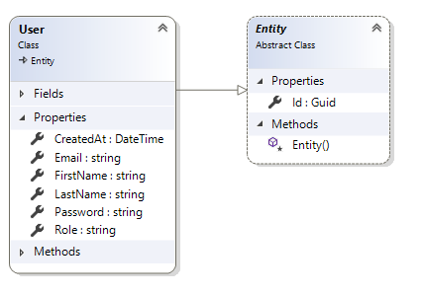
\includegraphics[width=.9\linewidth]{images/chapter_3/ef-code.png}
      \caption{Kod klasy User (\Csharp)}
      \label{fig:ef-code}
    \end{subfigure}%
    \begin{subfigure}{.4\textwidth}
      \centering
      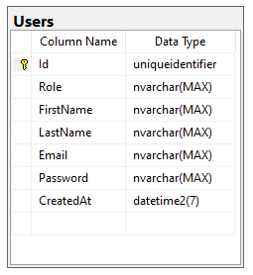
\includegraphics[width=.9\linewidth]{images/chapter_3/ef-db.png}
      \caption{Tabela Users w bazie danych}
      \label{fig:ef-db}
    \end{subfigure}
    \caption{Mapowanie klas na struktury bazodanowe}
    \label{fig:ef}
\end{figure}
    
Projekt został zrealizowany według pierwszego podejścia: Code First. Przygotował on Domenę, którą następnie za pomocą migracji odwzorował na nowo utworzonej bazie danych. 

%%%%%%%%%%%%%%%%%%%%%%%%%%%%%%%%%%%%%%%%%%%%%%%%%%%%%%%%%%%%
%% JWT
%%%%%%%%%%%%%%%%%%%%%%%%%%%%%%%%%%%%%%%%%%%%%%%%%%%%%%%%%%%% 
\subsubsection{JWT}
JSON Web Token (w skrócie JWT) to otwarty standard (RFC 7519), który odpowiada za wymianę danych pomiędzy stronami (klient-serwer) w bezpieczny sposób poprzez obiekt w formacie JSON. Informacje przekazywane w nim mogą zostać zweryfikowane przy użyciu cyfrowego podpisu, który jest zawarty w tokenie. Podpis jest generowany za pomocą algorytmu HMAC lub klucza publicznego/prywatnego RSA lub ECDSA.
    
JWT może zostać wykorzystany przy:
\begin{itemize}
    \item Autoryzacji
    \item Transmisji danych
\end{itemize}
    
Struktura JWT, w swojej wynikowej postaci, składa się z trzech części oddzielonych kropkami. Są to kolejno nagłówek (ang. Header), zawartość (ang. Payload), podpis (ang. Signature). Podział ten jest pokazany na rysunku \ref{fig:jwt}
    
\begin{figure}[H] 
    \centering
    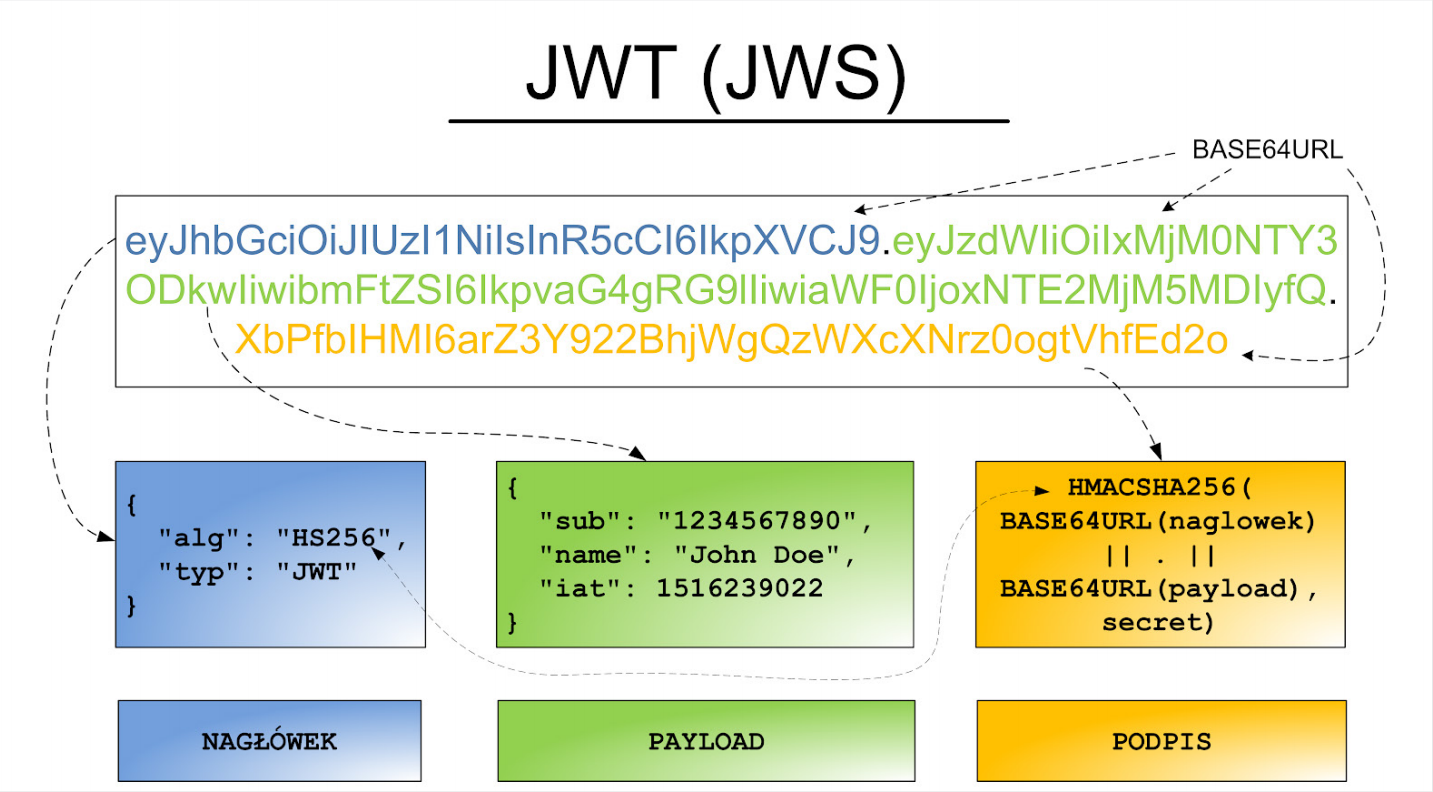
\includegraphics[width=1\textwidth]{images/chapter_3/jwt.png}
    \caption{Przykład podstawowego JWT \cite{sekurak-jwt}}
    \label{fig:jwt}
\end{figure}
    
    \myparagraph{Nagłówek}
    \begin{figure}[H] 
     	\centering
    	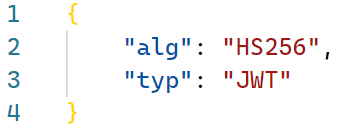
\includegraphics[width=0.4\textwidth]{images/chapter_3/jwt-header.png}
    	\caption{Przykład nagłówka tokenu}
    	\label{fig:jwt-header}
    \end{figure}
    
    Nagłówek (pokazany na rysunku \ref{fig:jwt-header}) zawiera dwie informację: rodzaj tokena np. JWT oraz jaki algorytm został użyty do wygenerowania podpisu np. HMAC-SHA256 (zapisywany jako HS256). W postaci końcowej (token), nagłówek jest zapisywany za pomocą algorytmu BASE64URL.
    
    \myparagraph{Zawartość}
    \begin{figure}[H] 
     	\centering
    	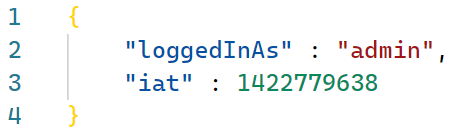
\includegraphics[width=0.6\textwidth]{images/chapter_3/jwt-payload.png}
    	\caption{Przykład zawartości tokenu}
    	\label{fig:jwt-payload}
    \end{figure}
    
    Środkowa cześć jest odpowiedzialna za przechowywanie danych, które chcemy zawrzeć w tokenie. Są to roszczenia (ang. claims). Specyfikacja JWT definiuje siedem zarejestrowanych roszczeń. Roszczenia niestandardowe są często wykorzystywane, w zależności od celu tokena.
    Przykład pokazany na rysunku \ref{fig:jwt-payload} pokazuje \textit{Issued At Time, "iat"} czyli datę wydania roszczenia i roszczenie niestandardowe \textit{loggedInAs}.
    
    Zawartość również jest kodowana za pomocą algorytmu BASE64URL.
    \clearpage
    \myparagraph{Podpis}
    \label{signature}

    \begin{figure}[H] 
     	\centering
    	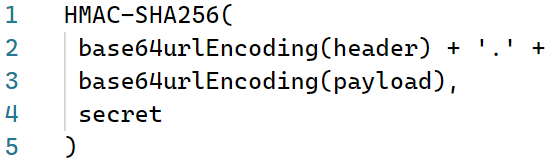
\includegraphics[width=0.5\textwidth]{images/chapter_3/jwt-signature.png}
    	\caption{Sposób obliczania podpisu}
    	\label{fig:jwt-signature}
    \end{figure}
    
    Podpis cyfrowy potwierdza autentyczność danych zapisanych w tokenie. Walidacja podpisu daje nam gwarancje że nadawca wiadomości jest tym za kogo się podaje.
    
    Podpis haszowany jest za pomocą wybranego algorytmu (w pokazanym przykładzie - rysunek \ref{fig:jwt-header} był to HMAC-SHA256). Do tej procedury potrzebujemy trzech danych: zakodowanego nagłówka za pomocą algorytmu BASE64URL, zakodowanej zawartości za pomocą algorytmu BASE64URL i sekretu. 
    
    Sekret to mówiąc najprościej hasło. Serwis autoryzacyjny (w naszym przypadku serwer z API) przechowuje takie hasło i wykorzystuje przy generowaniu całego tokenu. Hasło musi być tajne, a jego kompromitacja oznacza że każdy może wygenerować taki token i przejść autoryzacje w naszym portalu.
    
    \begin{figure}[H] 
     	\centering
    	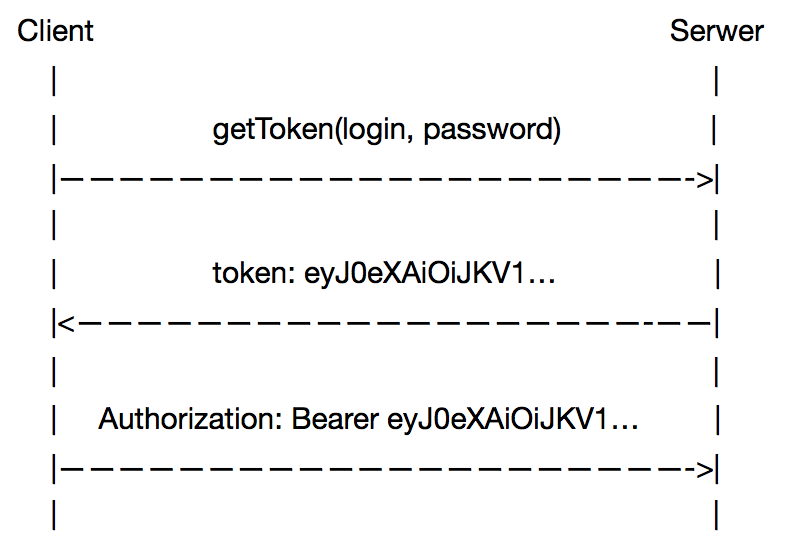
\includegraphics[width=0.8\textwidth]{images/chapter_3/token-diagram.png}
    	\caption{Działanie tokenu w praktyce \cite{token-diagram}}
    	\label{fig:token-diagram}
    \end{figure}
    
    Rysunek \ref{fig:token-diagram} pokazuje trzy akcje:
    \begin{enumerate}
        \item Logowanie (proces uzyskania tokenu), klient przesyła login i hasło
        \item Serwer (\textit{Find-A-Tutor.API}) po pomyślnym zweryfikowaniu danych, generuje token JWT zgodnie z algorytmem pokazanym w tym rozdziale. Zwraca go jako odpowiedź do poprzedniego zapytania (logowanie)
        \item Użytkownik podczas wysyłania zapytania do API przekazuje także wcześniej otrzymany token. Jeśli token jest poprawny, serwer zwróci odpowiedni dane. Jeśli nie, zwróci komunikat o nieprawidłowym tokenie (lub o jego wygaśnięciu)
    \end{enumerate}
    
%%%%%%%%%%%%%%%%%%%%%%%%%%%%%%%%%%%%%%%%%%%%%%%%%%%%%%%%%%%%
%% Swagger UI
%%%%%%%%%%%%%%%%%%%%%%%%%%%%%%%%%%%%%%%%%%%%%%%%%%%%%%%%%%%% 
\subsubsection{Swagger UI}
Swagger to otwarty framework wspierany przez duży ekosystem narzędzi który pomaga programistom projektować, budować, dokumentować i użytkować WebApi. 
Swagger UI pozwala na wizualizacje WebApi. Użytkownik ma możliwość zapoznać się ze wszystkimi endpointami (adresami) pod które może kierować zapytania. Widzi on jakie są dostępne kontrolery oraz jakie akcje udostępnia. Rysunek \ref{fig:swagger} pokazuje akcje dla dwóch kontrolerów (PrivateLesson i SchoolSubject). 
    
\begin{figure}[H] 
    \centering
    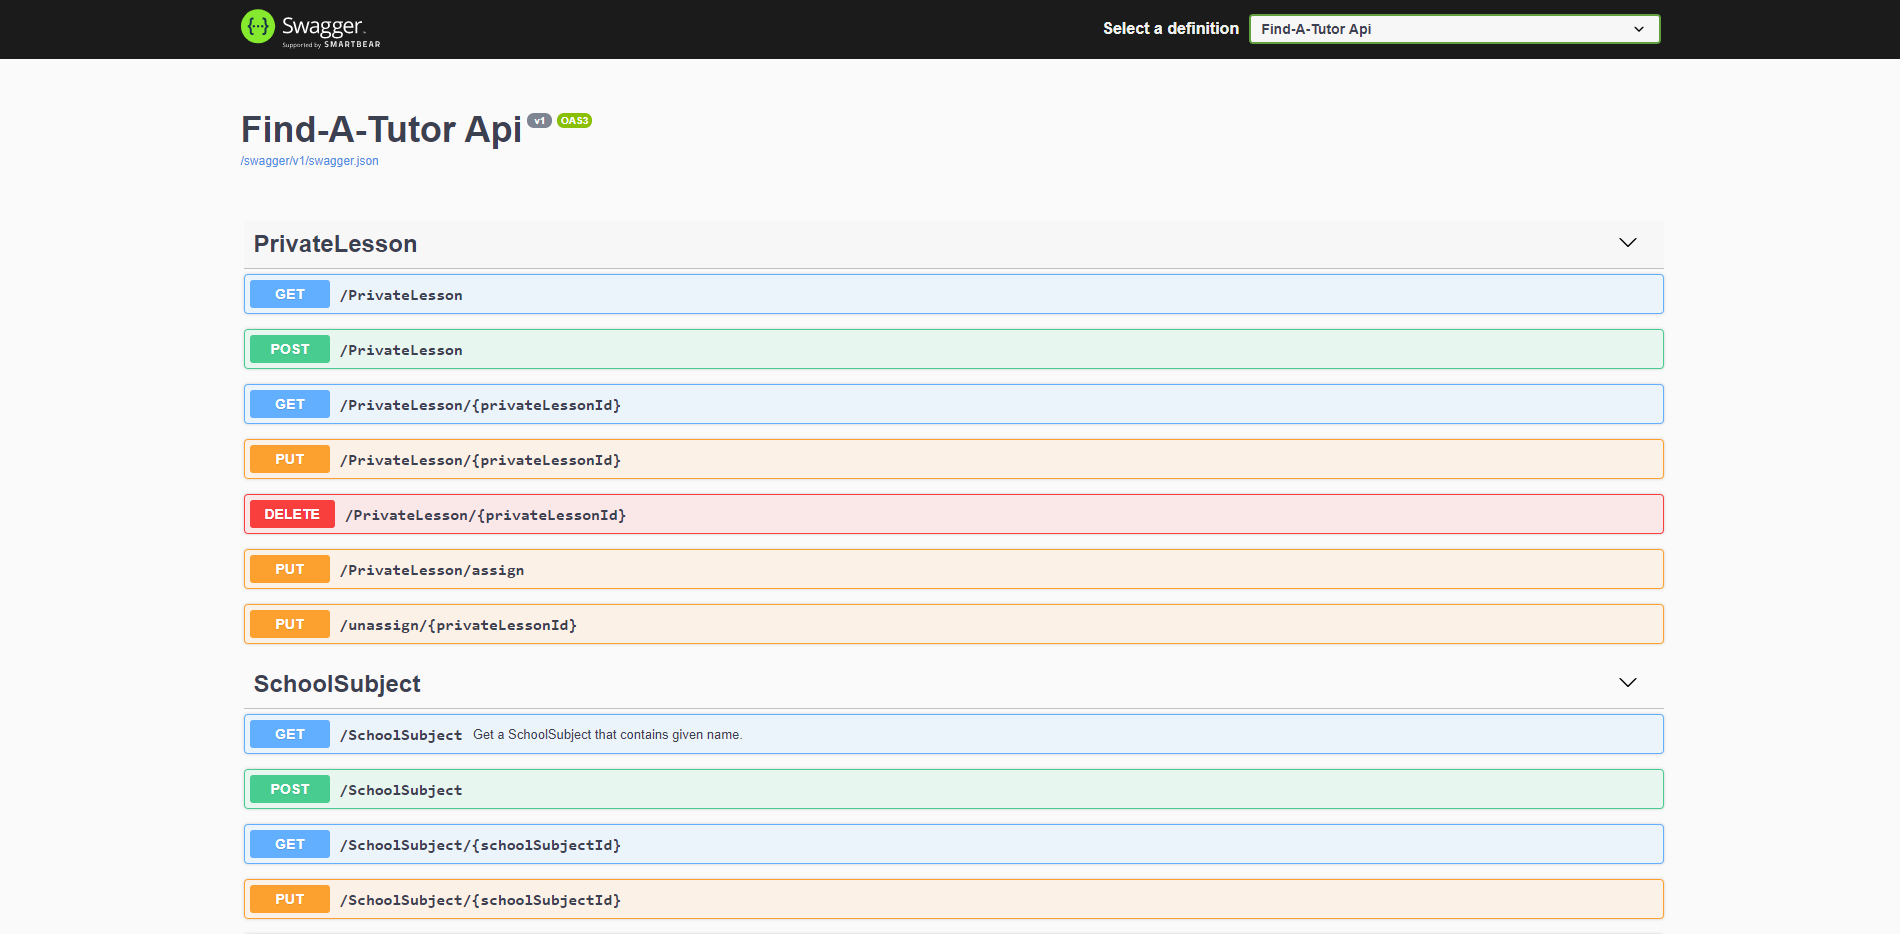
\includegraphics[width=1\textwidth]{images/chapter_3/swagger.png}
    \caption{Interfejs Swagger UI dla aplikacji \textit{Find-A-Tutor}}
    \label{fig:swagger}
\end{figure}
    
Dodatkowo, użytkownik ma możliwość przetestowania każdego zapytania, a także zapoznania się z możliwymi odpowiedziami serwera (wraz z modelem), opisem i nazwą argumentów. Na rysunku \ref{fig:swagger-get}, jest to zapytanie \textbf{GET} o listę wszystkich przedmiotów szkolnych. 
    
\begin{figure}[H] 
    \centering
    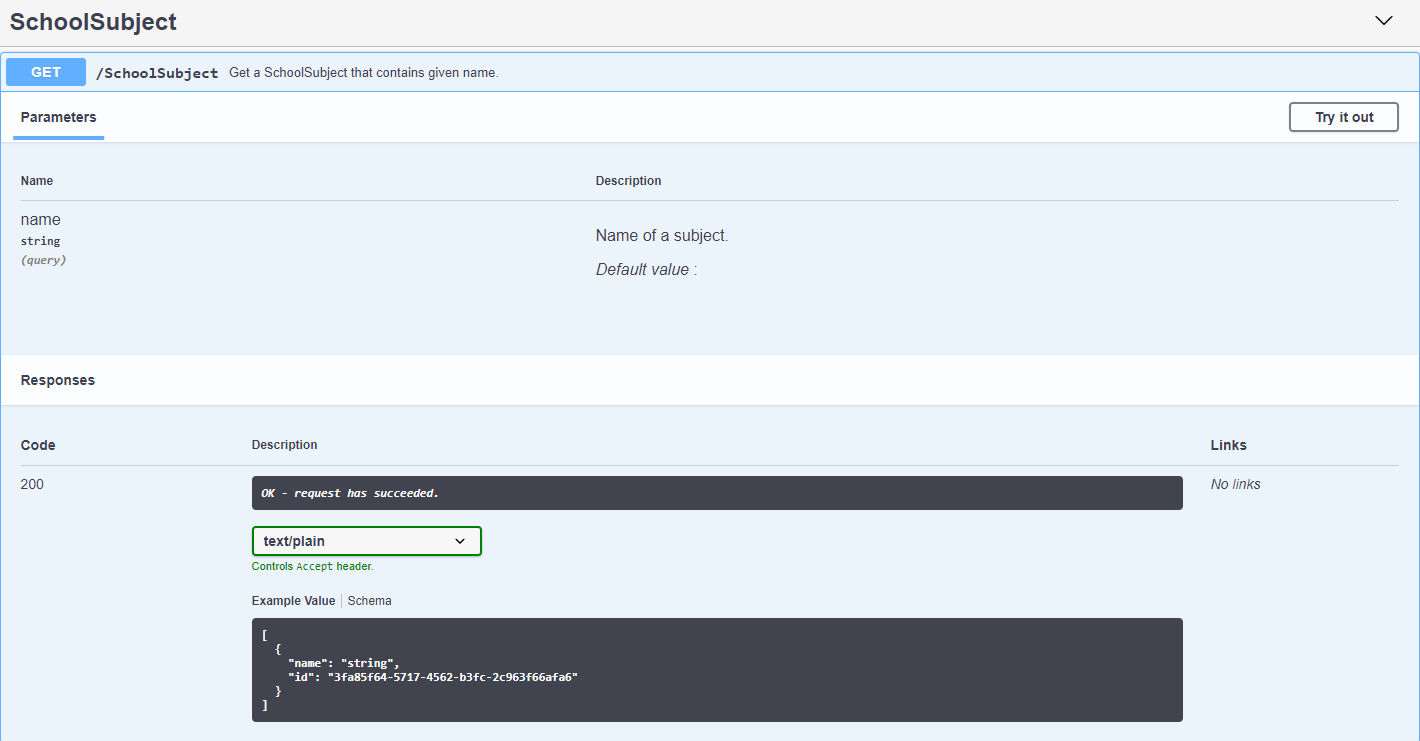
\includegraphics[width=1\textwidth]{images/chapter_3/swagger-get.png}
    \caption{Szczegóły zapytania GET}
    \label{fig:swagger-get}
\end{figure}
    
Panel Swagger UI jest dostępny pod adresem /swagger.
% \subsubsection{NLog}
% \subsubsection{Automapper}
% \subsubsection{Figgle}

%%%%%%%%%%%%%%%%%%%%%%%%%%%%%%%%%%%%%%%%%%%%%%%%%%%%%%%%%%%%
%% Architektura aplikacji - Backend
%%%%%%%%%%%%%%%%%%%%%%%%%%%%%%%%%%%%%%%%%%%%%%%%%%%%%%%%%%%% 
\subsection{Architektura aplikacji - Backend}
    
Aplikacje które są zgodne z \textit{Zasadą Odwrócenia Zależności} (ang. Dependency Inversion Principle), a także z zasadami projektowania opartego na domenie (ang. Domain-Driven Design - DDD) mają tendencję do uzyskiwania podobnej architektury. Ta architektura na przestrzeni lat nosiła wiele nazw. Jedną z pierwszych nazw była \textit{Architektura Heksagonalna} (ang. Hexagonal Architecture), a następnie \textit{Porty I Adaptery} (ang. Ports-and-Adapters). Co raz częściej nazywa się ją \textit{Architekturą Cebulową} (ang. Onion Architecture) lub \textit{Czystą Architekturą} (ang. Clean Architecture). Autor w swojej pracy używa właśnie tej drugiej nazwy.

\textit{Czysta Architektura} stawia logikę biznesową i model aplikacji w środku aplikacji. Zamiast uzależniania logiki biznesowej od dostępu do danych lub innych problemów związanych z infrastrukturą, zależność ta jest odwrócona: szczegóły infrastruktury i jej implementacji zależą od rdzenia aplikacji. Osiąga się to poprzez zdefiniowanie interfejsów lub abstrakcji w rdzeniu aplikacji, które są następnie implementowane przez typy zdefiniowane w warstwie infrastruktury. Należy podkreślić że poprawnie wymodelowana domena nie posiada żadnych referencji do innych warstw aplikacji.
    
Częstym sposobem wizualizacji tej architektury jest użycie szeregu koncentrycznych kół, podobnych do cebuli. Rysunek \ref{fig:clean-architecture} pokazuje \textit{Czystą Architekturę} przy użyciu tego stylu reprezentacji architektonicznej. Nazwa \textit{Cebulowa Architektura} zawdzięcza nazwę właśnie takiemu ułożeniu warstw.
    
\begin{figure}[H] 
    \centering
    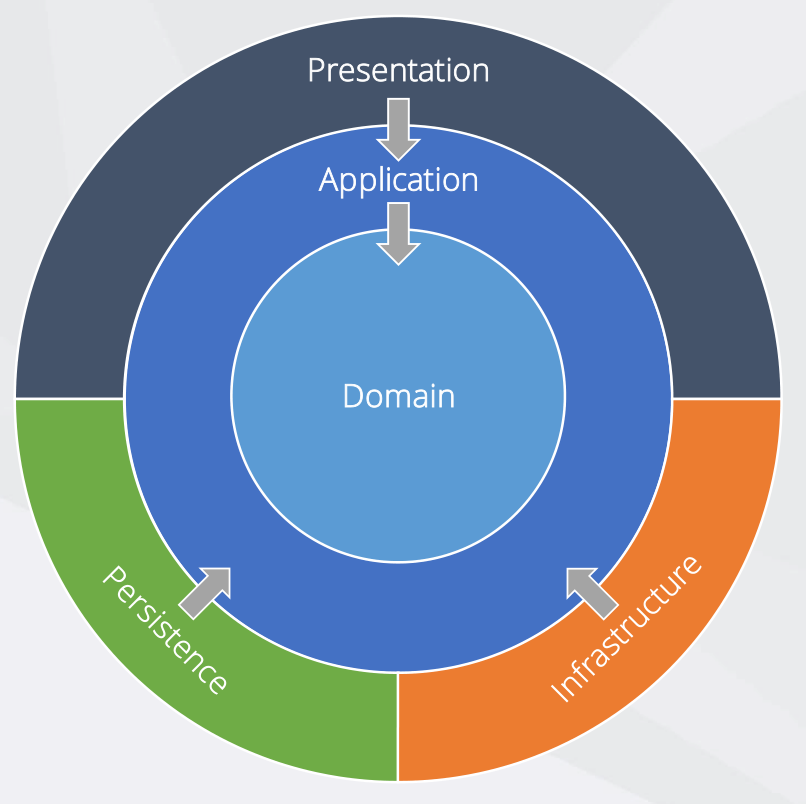
\includegraphics[width=0.7\textwidth]{images/chapter_3/clean-architecture.png}
    \caption{Czysta Architektura \cite{clean-architecture}. Każda warstwa jest zależna od warstwy bliżej centrum - aż do domeny która nie ma żadnych zależności. Warstwa aplikacji zależy od warstwy domeny, a pozostałe trzy (prezentacji, infrastruktury i utrwalenia) zależy od warstwy aplikacji.}
    \label{fig:clean-architecture}
\end{figure}
    
Autor w swoim projekcie zastosował właśnie takie rozwiązanie, ze względu na czystość, prostotę implementacji, łatwość zmian (np. wymiany infrastruktury na zupełnie nową) i przede wszystkim czytelność \cite{clean-architecture}. 

    \subsubsection{Rdzeń} \label{core}
    Centralnym elementem architektury jest rdzeń. Składa się on z \textit{Warstwy domeny} i \textit{Warstwy aplikacji}, pokazanej na rysunku \ref{fig:clean-architecture}. Obie te warstwy zawierają logikę biznesową i logikę aplikacji (wraz z zdefiniowanymi typami). 
        
    Zgodnie z \textit{PI} (ang. Persistence Ignorance) i \textit{Zasadą Ignorowania Infrastruktury} (ang.  Infrastructure Ignorance) ta warstwa musi całkowicie ignorować szczegóły dotyczące trwałości danych (np. zapis i odczyt). Te zadania powinny zostać wykonane przez warstwę infrastruktury. Dlatego ta warstwa nie powinna przyjmować bezpośrednich zależności od infrastruktury, co oznacza że ważne jest aby klasy reprezentujące encję modelowe były obiektami POCO.
        
    Domenowe encję nie powinny mieć żadnej bezpośredniej zależności (jak dziedziczenie) do frameworka służącego do dostępu danych jak np. Entity Framework (technologia szczegółowo opisana w rozdziale \ref{EF}).
        
    %\paragraph{Wzorzec repozytorium}
    \subsubsection{Infrastruktura}
    Warstwa infrastruktury i utrwalenia (ang. persistence) opisuje sposób w jaki dane które są początkowo trzymane w klasach modelowych (w pamięci) są utrwalane w bazie danych lub w jakiejkolwiek innej postaci. Przykładem takiego utrwalenia (który Autor zaimplementował) jest Entity Framework Core. Napisany kod służy do połączanie się z bazą danych przez DBContext, który jest reprezentacją bazy danych jako obiekt. Dzięki temu w łatwy sposób możemy operować danymi w naszej bazie danych.
        
    Ta warstwa zależy od warstw niżej - aplikacji i domeny.
        
    \subsubsection{API}
    Warstwą odpowiedzialną za kontakt "na zewnątrz" jest warstwa prezentacji. W projekcie backendowym, zaimplementowana zostało ona jako WebApi, wraz z najpopularniejszym stylem architektury REST. Za format wymiany danych posłużył JSON.
        
        \myparagraph{RESTful WebAPI}
        WebApi jest to aplikacja z którą komunikacja jest ograniczona do protokołu HTTP. Protokół ten zawiera 9 metod przy pomocy których możemy sterować WebApi. 
        HTTP jest niezależny od platformy i jest bezstanowy - nie zachowuje żadnych informacji poprzednich transakcjach z klientem). 
        
        Aplikacja taka wystawia na świat adresy URL, dalej zwane endpointami.
        Endpointy są rdzeniem aplikacji WebAPI. To właśnie do nich użytkownik końcowy kieruje zapytania. Jako przykładem, Autor posłuży się następującym endpointem - \textbf{http://domena/privatelesson/3}. Użytkownika interesuje zasób "privatelesson" o ID równym 3. Korzystając z jednej metod protokołu HTTP - GET, wysyłamy owe zapytanie.
        
        Gdyby użytkownik skorzystał z metody PUT, mógłby on zaktualizować dane znajdujące się pod tym endpointem. Wszystkie metody są opisane przez dokument \textbf{RFC2616} \cite{http}.
        
        REST (ang. Representational State Transfer) jest wzorcem architektonicznym który narzuca dobre praktyki przy tworzeniu aplikacji.
        RESTful WebAPI to WebApi które stosuje się do zasad wzorca REST i jest zaimplementowane na bazie protokołu HTTP.
        
        \myparagraph{JSON}
        \indent
        \textbf{JavaScript Object Notation}, w skrócie JSON to otwarty i lekki format wymiany danych komputerowych. Charakteryzuje się tekstem czytelnym dla człowieka. Używany jest do przesyłania obiektów danych składających się z par atrybut-wartość i tablicowych typów danych (lub każdej innej wartości możliwej do serializacji) \cite{json}.
        
        Sam zapis jest dokonywany tylko przy użyciu sześciu znaków: \{, \}, [, ], : (dwukropek) oraz , (przecinek). Proces ten został zwizualizowany na rysunku \ref{fig:json}.
        
        \begin{figure}[H] 
         	\centering
        	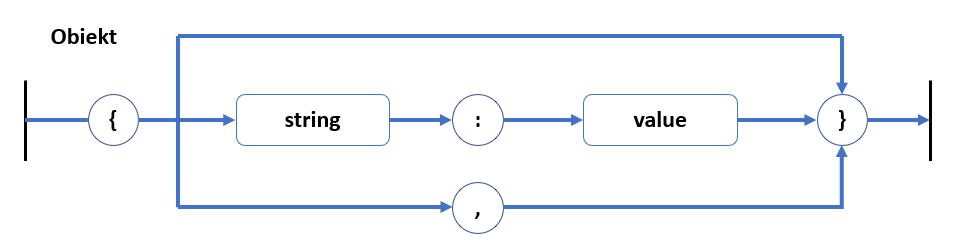
\includegraphics[width=1.0\textwidth]{images/chapter_3/json.png}
        	\caption{Schemat zapisu danych typu obiekt w formacie JSON}
        	\label{fig:json}
        \end{figure}
        
        JSON jest niezależny od języka. Został zaczerpnięty z JavaScriptu, ale prawie wszystkie nowoczesne języki programowania zawierają funkcjonalność generowania i parsowania danych sformatowanych za pomocą JSONa. Dlatego też stał się on uniwersalnym formatem do deserializacji danych, przesyłania ich do/z WebApi, jak i nawet przechowywaniu ich na dysku.
        
        W \textit{Find-A-Tutor} stał się on jednym formatem wymiany danych - WebAPI, przyjmuje i zwraca dane w JSONie. 
        
        \begin{figure}[H] 
         	\centering
        	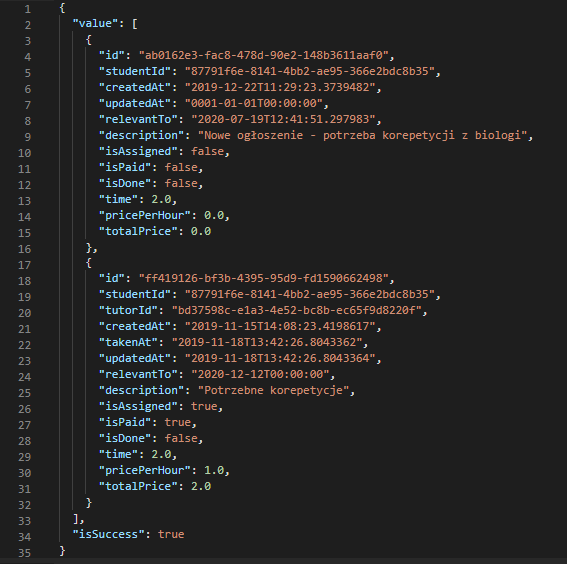
\includegraphics[width=.8\textwidth]{images/chapter_3/json-get.png}
        	\caption{Rezultat wysłanego zapytania do WebAPI}
        	\label{fig:json-get}
        \end{figure}
        
        Na rysunku \ref{fig:json-get} pokazany jest rezultat zapytania metodą GET do WebApi. Są to wszystkie ogłoszenia danego użytkownika (dodane z jego konta).
        
%%%%%%%%%%%%%%%%%%%%%%%%%%%%%%%%%%%%%%%%%%%%%%%%%%%%%%%%%%%%
%% Architektura aplikacji - Frontend
%%%%%%%%%%%%%%%%%%%%%%%%%%%%%%%%%%%%%%%%%%%%%%%%%%%%%%%%%%%% 
\clearpage
\subsection{Architektura aplikacji - Frontend}
Najmniejsza możliwa liczba projektów dla architektury aplikacji to jeden. W takiej aplikacji, cała logika jest zawarta w jednym projekcie, kompilowana do jednego pliku wykonywalnego i wdrożona jako jedna całość. 
    
Ze względu na podział backend - frontend, to właśnie API (backend) odpowiada za faktyczną logikę projektu. I to przez ten interfejs, aplikacja frontendowa porozumiewa się z serwerem czy bazą danych. 
    
W praktyce każda akcja wykonana na froncie (np. logowanie, pobieranie danych) odbywa się poprzez wysłanie odpowiedniego zapytania do API. 
    
\subsubsection{MVC}
Model–view–controller (pol. Model-Widok-Kontroler), to wzorzec architektoniczny powszechnie używany do opracowania aplikacji posiadających graficzne interfejsy użytkownika. 

\begin{figure}[H] 
    \centering
    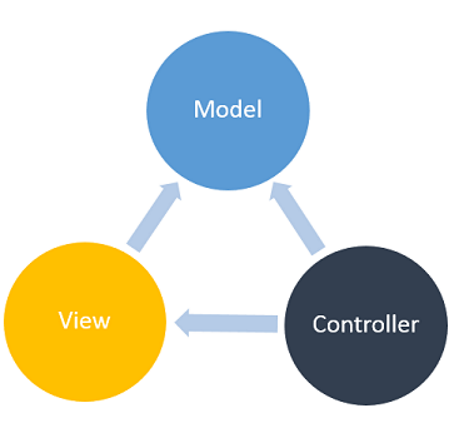
\includegraphics[width=.5\textwidth]{images/chapter_3/mvc.png}
    \caption{ Model-Widok-Kontroler \cite{mvc}}
    \label{fig:mvc}
\end{figure}
    
MVC dzieli aplikacje na trzy części:
\begin{itemize}
    \item Model - logika biznesowa
    \item Widok - graficzne interfejsy dla użytkownika (UI od ang. user interface) 
    \item Kontroler - obsługuje żądania użytkownika i konwertuje je na polecenia widoku lub modelu
\end{itemize}
    
Wszystkie jego części są ze sobą połączone, pokazuje to rysunek \ref{fig:mvc}.
Aplikacja frontendowa została zaprojektowana używając właśnie tej architektury. 
Prześledźmy zatem pojedynczą akcję użytkownika - logowanie:
\begin{enumerate}
    \item Użytkownik zostaje zwrócony odpowiedni UI (Widok)
    \item Użytkownik wpisuje w pola login i hasło 
    \item Aplikacja obsługuje te dane i przekazuje dalej (Kontroler)
    \item Aplikacja opakowuje owe dane (JSON) i wysyła jako zapytanie HTTP do WebApi (Model)
        \begin{itemize}
            \item WebApi otrzymuje dane i je przetwarza, cały proces został opisany w rozdziale \ref{signature}
        \end{itemize}
    \item WebApi zwraca dane do aplikacji, są one rozpakowywane, i przekazywane dalej (Model)
    \item Model aktualizuje Widok, co jest widoczne dla użytkownika
\end{enumerate}
    
Przepływ danych został pokazany na rysunku \ref{fig:mvc-flow}.
    
\begin{figure}[H] 
    \centering
    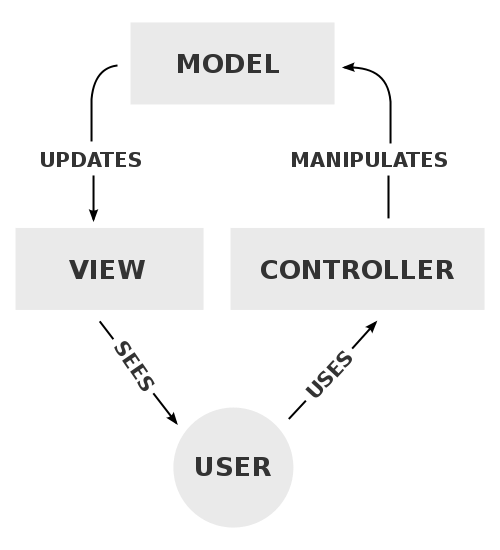
\includegraphics[width=.5\textwidth]{images/chapter_3/mvc-flow.png}
    \caption{Zasada organizacji MVC \cite{mvc-flow}}
    \label{fig:mvc-flow}
\end{figure}
    
Przedstawiony scenariusz pokazuje że frontend został napisany na zasadach klienta który obsługuje żądania użytkownika i usprawnia (np. przez UI) komunikacje użytkownika z serwerem. 
Rozdzielenie tych dwóch projektów ma następujące zalety:
\begin{itemize}
    \item Modularność - w razie potrzeby jesteśmy wstanie wymienić jeden z projektów na inny
    \item W razie zmiany popularny stylów graficznych, można w łatwy sposób napisać sam frontend od nowa, dzięki czemu cała aplikacja zostaje nietknięta
    \item Ułatwienie w utrzymaniu i pracy nad projektem
    \item Możliwość pracy w dwóch osobnych zespołach na obu projektach
\end{itemize}
    
% \subsubsection{Razor Pages}

%%%%%%%%%%%%%%%%%%%%%%%%%%%%%%%%%%%%%%%%%%%%%%%%%%%%%%%%%%%%
%% Warstwa bazy danych
%%%%%%%%%%%%%%%%%%%%%%%%%%%%%%%%%%%%%%%%%%%%%%%%%%%%%%%%%%%% 
\subsection{Warstwa bazy danych}
Ze względu na charakterystykę aplikacji, Autor zdecydował się na bazę relacyjną.
Zgodnie z wymodelowaną domeną opisaną w rozdziale \ref{core} i korzystając z mappera obiektowo-relacyjnego (EF Core) opisanego w rozdziale \ref{EF}, struktura bazodanowa została wygenerowana za pomocą migracji. Autor zastosował obsługiwany sposób Code First, czyli na podstawie kodu, EF wygenerował model bazodanowy.
    
Dodatkowo, Autor wybrał \textit{Microsoft SQL Server} jako silnik bazodanowy, mając na uwadze że i owy silnik, jak i platforma .Net Core (wraz z \Csharp) została opracowana przez firmę Microsoft. 
    
Poniżej, rysunek \ref{fig:db} przedstawia strukturę bazodanową: 
\begin{figure}[H] 
    \centering
    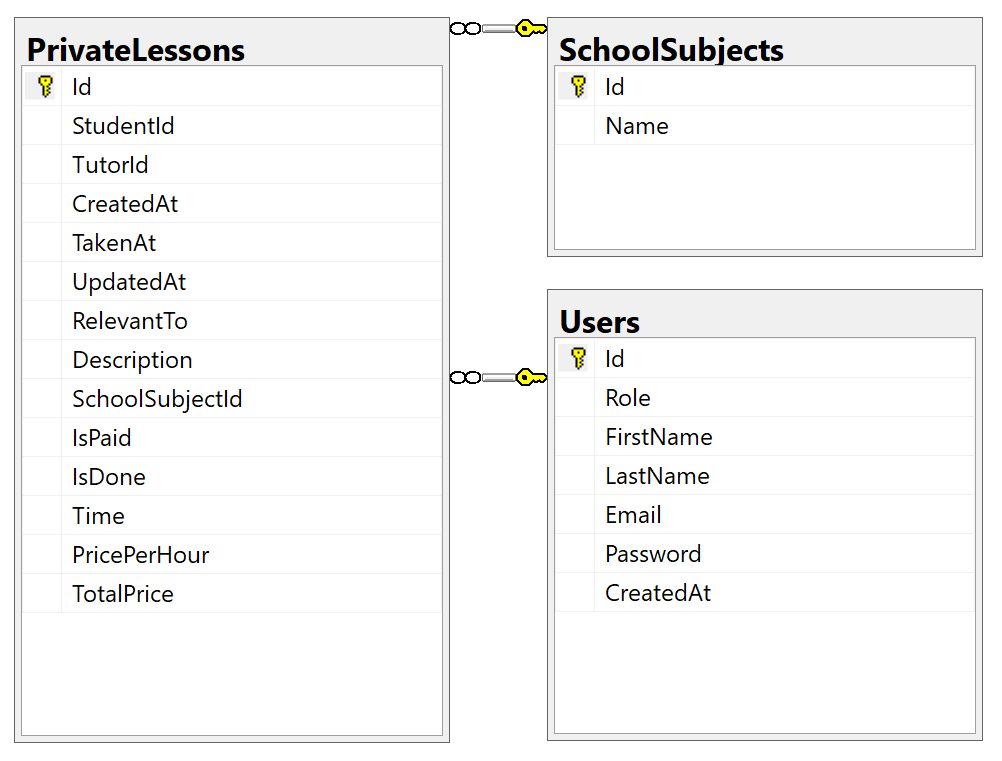
\includegraphics[width=.8\textwidth]{images/chapter_3/db.png}
    \caption{Struktury bazodanowe aplikacji \textit{Find-A-Tutor}}
    \label{fig:db}
\end{figure}
    
\textit{Podczas powstawania aplikacji Find-A-Tutor Autor postarał się aby była ona od samego początku dobrze zaprojektowana tak aby później modyfikacje nie komplikowały nadmiernie projektu. }

%%%%%%%%%%%%%%%%%%%%%%%%%%%%%%%%%%%%%%%%%%%%%%%%%%%%%%%%%%%%
%% Aplikacja z poziomu użytkownika
%%%%%%%%%%%%%%%%%%%%%%%%%%%%%%%%%%%%%%%%%%%%%%%%%%%%%%%%%%%%
\newpage
\section{Aplikacja z poziomu użytkownika}
W tym rozdziale pokazane zostało działanie aplikacji webowej \textit{Find-A-Tutor}. Zrzuty ekranu zostały wykonane w przeglądarce Chrome w wersji 79. Na rysunku \ref{fig:home} pokazany jest ekran startowy aplikacji.

\begin{figure}[!htbp] 
    \centering
    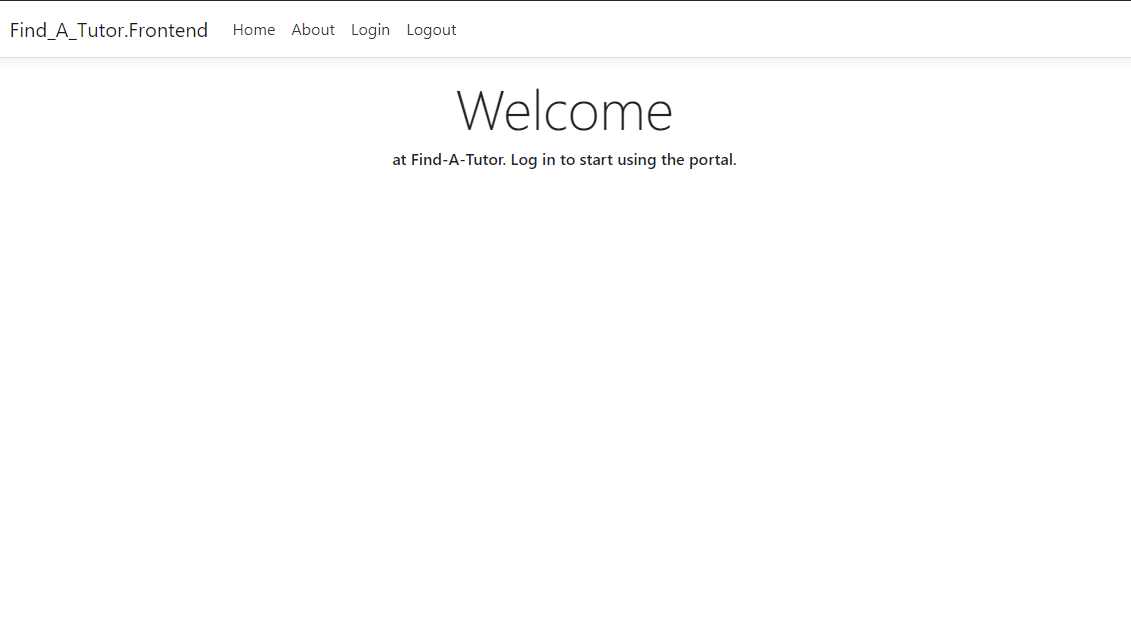
\includegraphics[width=1\textwidth]{images/chapter_4/home.png}
    \caption{Strona startowa aplikacji}
    \label{fig:home}
\end{figure}

%%%%%%%%%%%%%%%%%%%%%%%%%%%%%%%%%%%%%%%%%%%%%%%%%%%%%%%%%%%%
%% Uwierzytelnianie
%%%%%%%%%%%%%%%%%%%%%%%%%%%%%%%%%%%%%%%%%%%%%%%%%%%%%%%%%%%%
\subsection{Uwierzytelnianie}
Po kliknięciu "Login", użytkownikowi ukazuje się panel logowania (Rys. \ref{fig:login}
\begin{figure}[!htbp] 
    \centering
    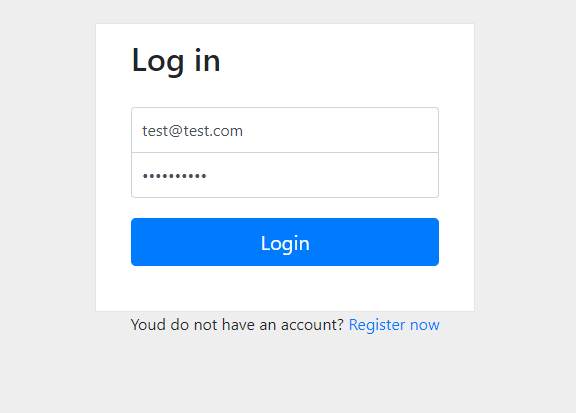
\includegraphics[width=0.7\textwidth]{images/chapter_4/login.png}
    \caption{Panel logowania}
    \label{fig:login}
\end{figure}

Po uzupełnieniu pól (mail i hasło) i wciśnięciu guzika "Login", dane są wysyłane do API. Jeśli uwierzytelnienie się powiodło, użytkownik jest przekierowywany do panelu użytkownika.

Jeśli użytkownik nie ma założonego konta, może to wykonać za pomocą linku "Register now", który przekierowuje go do podstrony z rejestracją - pokazaną na rysunku \ref{fig:register}.
\begin{figure}[!htbp] 
    \centering
    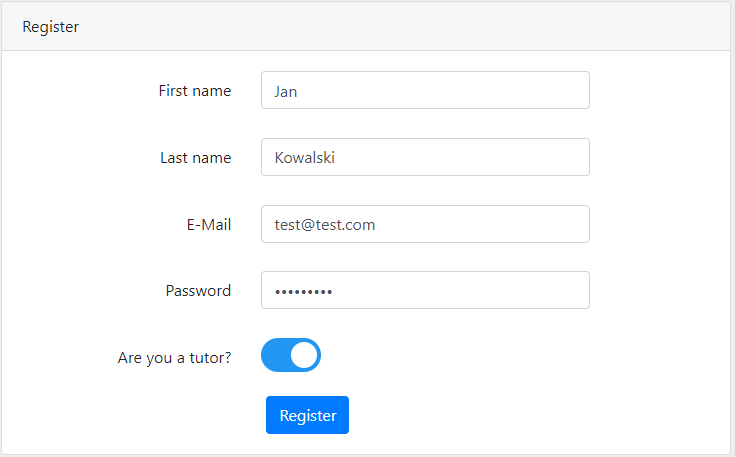
\includegraphics[width=1\textwidth]{images/chapter_4/register.png}
    \caption{Formularz rejestracji}
    \label{fig:register}
\end{figure}

Użytkownik ma do wypełnienia następujące pola: imię, nazwisko, adres email, hasło i typ konta (uczeń czy korepetytor). Poprawność danych sprawdzana jest w locie dzięki zastosowanym standardom (HTML 5) i po stronie serwera po kliknięciu guzika "Register".

%%%%%%%%%%%%%%%%%%%%%%%%%%%%%%%%%%%%%%%%%%%%%%%%%%%%%%%%%%%%
%% Panel użytkownika
%%%%%%%%%%%%%%%%%%%%%%%%%%%%%%%%%%%%%%%%%%%%%%%%%%%%%%%%%%%%
\subsection{Panel użytkownika}
\subsubsection{Dodanie nowego ogłoszenia}
Po pomyślnej uwierzytelnieniu użytkownika jako uczeń, wyświetlany jest mu panel użytkownika (Rysunek \ref{fig:student-empty}).
\begin{figure}[!htbp] 
    \centering
    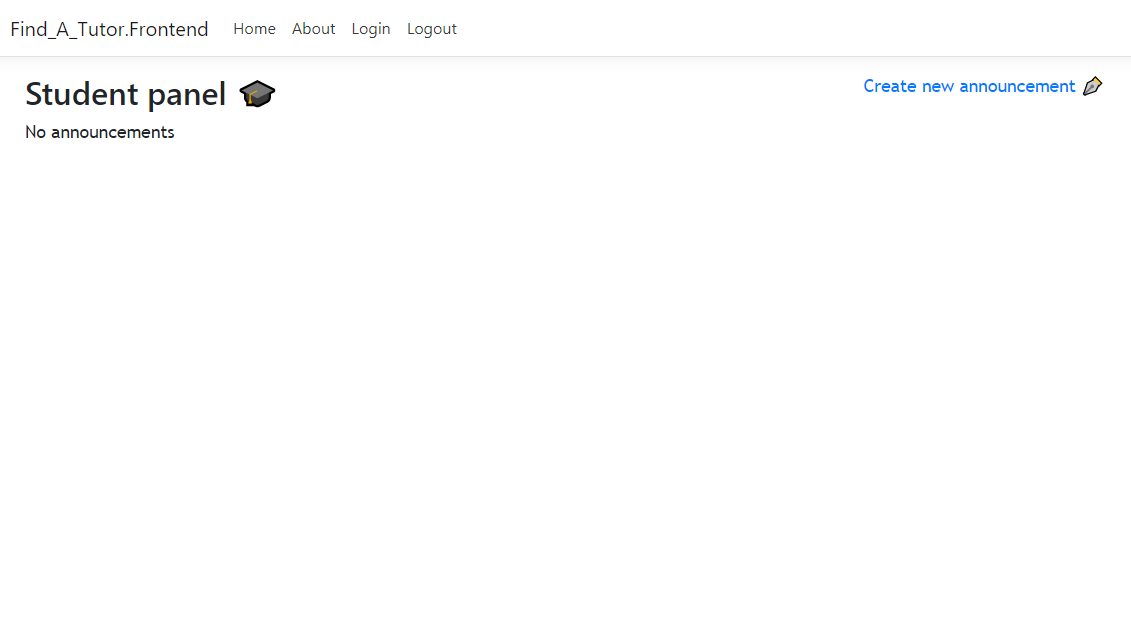
\includegraphics[width=1\textwidth]{images/chapter_4/student-empty.png}
    \caption{Pusty panel użytkownika}
    \label{fig:student-empty}
\end{figure}

Panel ten jest pusty. Aby dodać ogłoszenie, klikamy w link "Create new announcement" i zostajemy przekierowani do panelu dodawania nowego ogłoszenia, pokazany na rysunku \ref{fig:create-new}.
\begin{figure}[!htbp] 
    \centering
    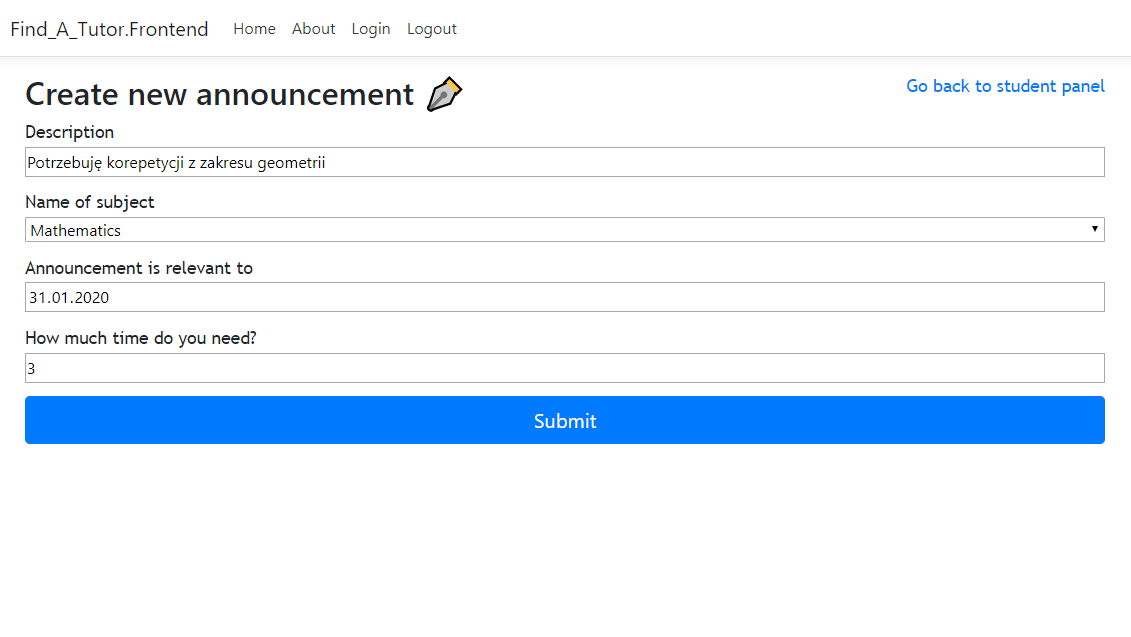
\includegraphics[width=1\textwidth]{images/chapter_4/create-new.png}
    \caption{Formularz do dodania nowego ogłoszenia}
    \label{fig:create-new}
\end{figure}

Użytkownik wypełnia tam następujące informacje: opis, datę ważności ogłoszenia i ile czasu będziemy potrzebować. Ponad to wybieramy przedmiot z listy. Kiedy dane są wpisane, użytkownik klika "Submit". Następuje ich wysłanie do API. Jeśli wszystko zostało poprawnie zwalidowane (np. data ważności nie jest datą historyczną), użytkownikowi pokaże się komunikat widoczny na rysunku \ref{fig:added}.
\begin{figure}[!htbp] 
    \centering
    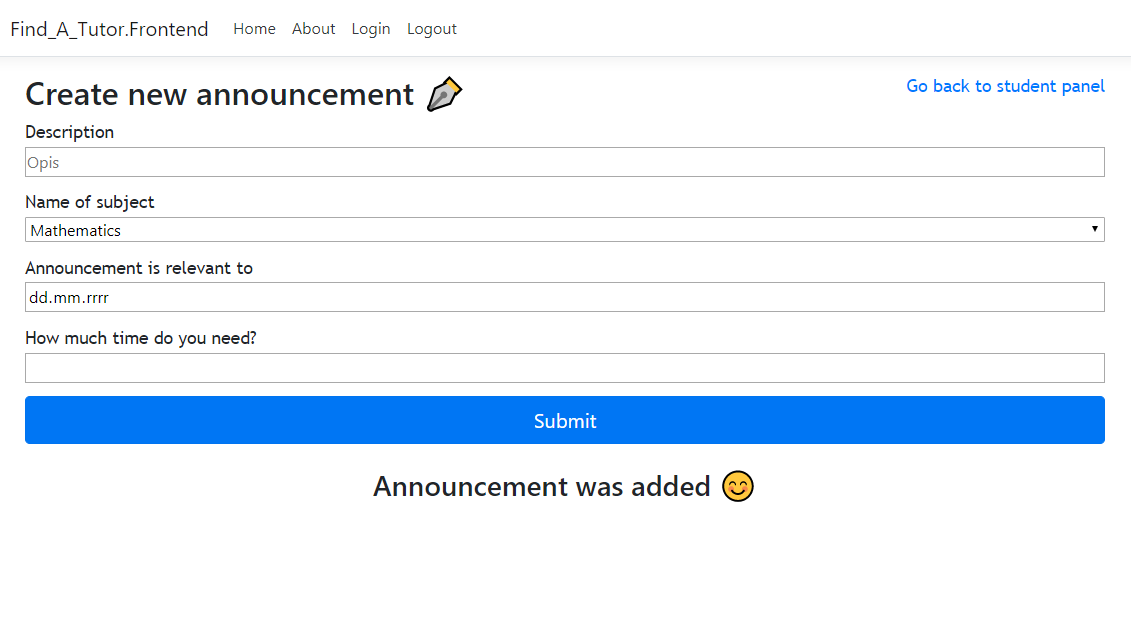
\includegraphics[width=1\textwidth]{images/chapter_4/added.png}
    \caption{Komunikat po dodaniu nowego ogłoszenia}
    \label{fig:added}
\end{figure}

Po wróceniu do panelu użytkownika, widoczne jest w nim dodane ogłoszenie (Rysunek \ref{fig:student}).
Widoczne są następujące informacje o nim: data utworzenia, datę podjęcia (na razie pustą), datę ważności, przedmiot, trzy flagi stanu (czy podjęta, czy zapłacona i czy wykonana) i link do podstrony z wszystkimi szczegółami ogłoszenia.
\begin{figure}[!htbp] 
    \centering
    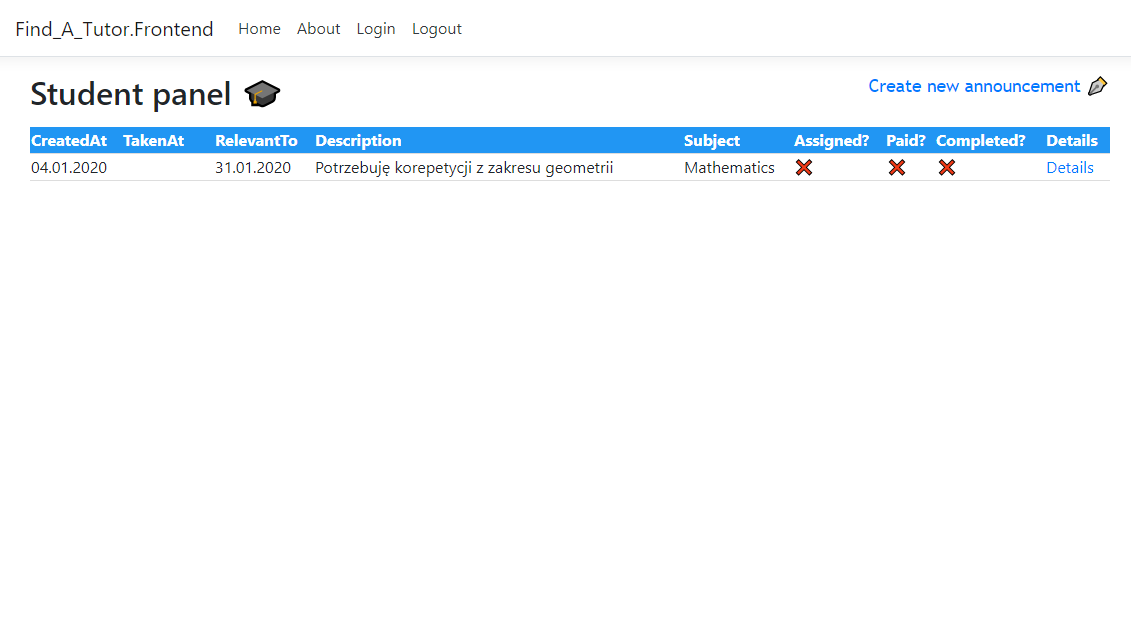
\includegraphics[width=1\textwidth]{images/chapter_4/student.png}
    \caption{Panel po dodaniu nowego ogłoszenia}
    \label{fig:student}
\end{figure}

%%%%%%%%%%%%%%%%%%%%%%%%%%%%%%%%%%%%%%%%%%%%%%%%%%%%%%%%%%%%
%% Podjęcie ogłoszenia
%%%%%%%%%%%%%%%%%%%%%%%%%%%%%%%%%%%%%%%%%%%%%%%%%%%%%%%%%%%%
\subsubsection{Podjęcie ogłoszenia}
Po pomyślnej uwierzytelnieniu użytkownika jako nauczyciel, jest mu wyświetlany panel nauczyciela (Rysunek \ref{fig:tutor-empty}).
\begin{figure}[!htbp] 
    \centering
    
\includegraphics[width=1\textwidth]{images/chapter_4/tutor-empty.png}
    \caption{Pusty panel nauczyciela}
    \label{fig:tutor-empty}
\end{figure}

Jeśli którykolwiek z uczniów dodał nowe ogłoszenie, jest ono tutaj wyświetlane (Rysunek \ref{fig:tutor}).
\begin{figure}[!htbp] 
    \centering
    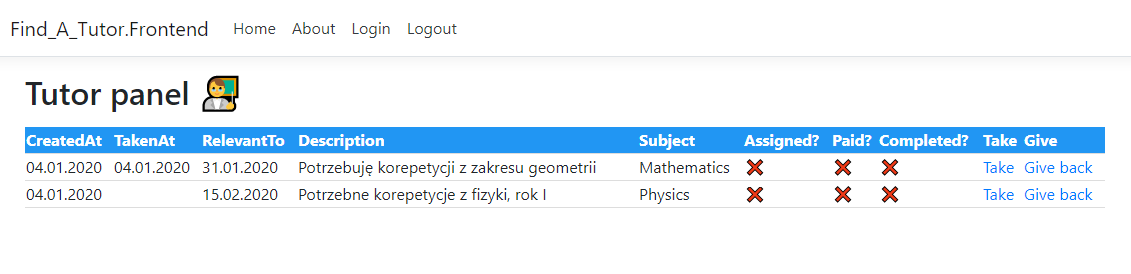
\includegraphics[width=1\textwidth]{images/chapter_4/tutor.png}
    \caption{Panel nauczyciela}
    \label{fig:tutor}
\end{figure}
Użytkownik może wykonać dwie akcje na ogłoszeniu - podjąć je lub oddać. Po naciśnięciu "Take", użytkownik zostaje przekierowany do podstrony ze szczegółami ogłoszenia (Rysunek \ref{fig:take}).

\begin{figure}[!htbp] 
    \centering
    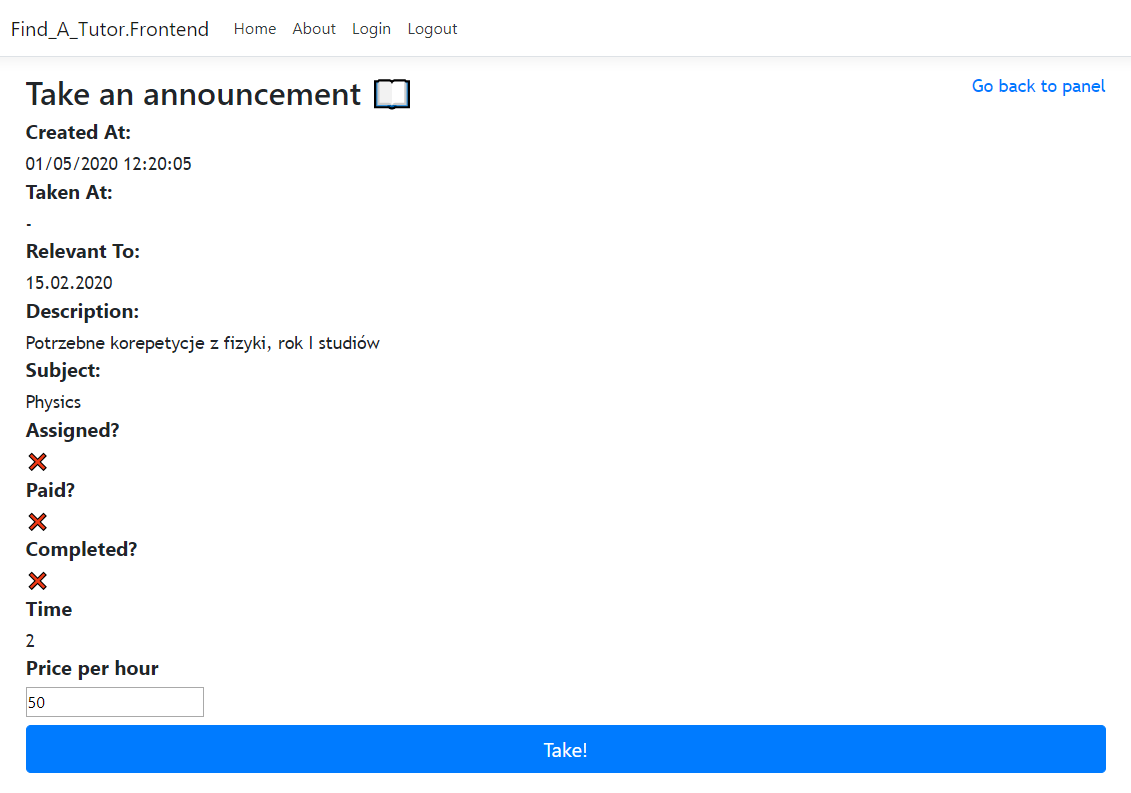
\includegraphics[width=1\textwidth]{images/chapter_4/take.png}
    \caption{Podjęcie ogłoszenia}
    \label{fig:take}
\end{figure}

W polu "Price per hour" użytkownik wpisuje stawkę godzinową. Po naciśnięciu guzika "Take", dana jest walidowana, przesłana, a ogłoszenie zostaje przypisane do konta nauczyciela.

Podjęcie może nastąpić tylko wtedy kiedy ogłoszenie jest wolne. Oddanie tylko wtedy kiedy jest przypisany do niego (użytkownik) i ogłoszenie nie zostało jeszcze opłacone.

Po powrocie do panelu użytkownika, widoczne jest w nim podjęte ogłoszenie wraz z oznaczeniem \cmark w polu "Czy przypisane" (Rysunek \ref{fig:tutor-assigned}).
\begin{figure}[!htbp] 
    \centering
    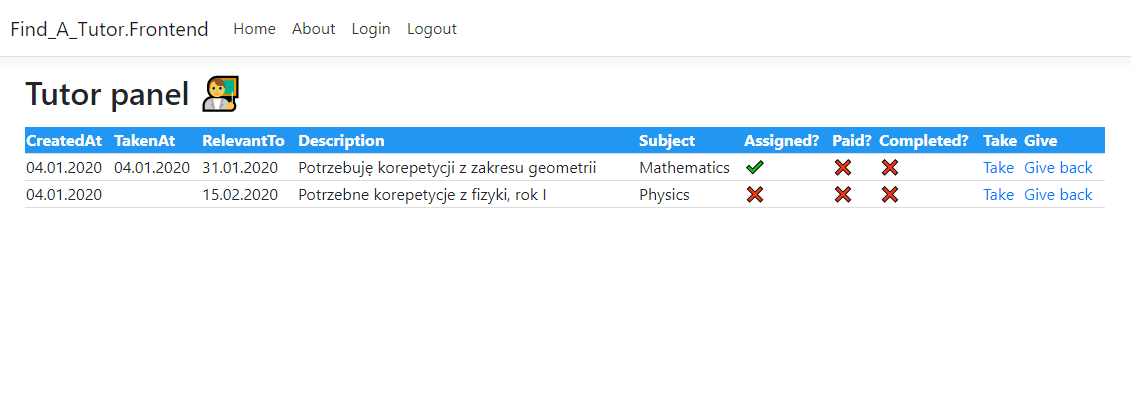
\includegraphics[width=1\textwidth]{images/chapter_4/tutor-assigned.png}
    \caption{Panel nauczyciela}
    \label{fig:tutor-assigned}
\end{figure}

%%%%%%%%%%%%%%%%%%%%%%%%%%%%%%%%%%%%%%%%%%%%%%%%%%%%%%%%%%%%
%% Płatność
%%%%%%%%%%%%%%%%%%%%%%%%%%%%%%%%%%%%%%%%%%%%%%%%%%%%%%%%%%%%
\subsubsection{Płatność}
Po ponownym zalogowaniu użytkownika (ucznia) widoczna jest zmiana w ogłoszeniu - zostało ono podjęte (Rysunek \ref{fig:student-assigned}).
\begin{figure}[!htbp] 
    \centering
    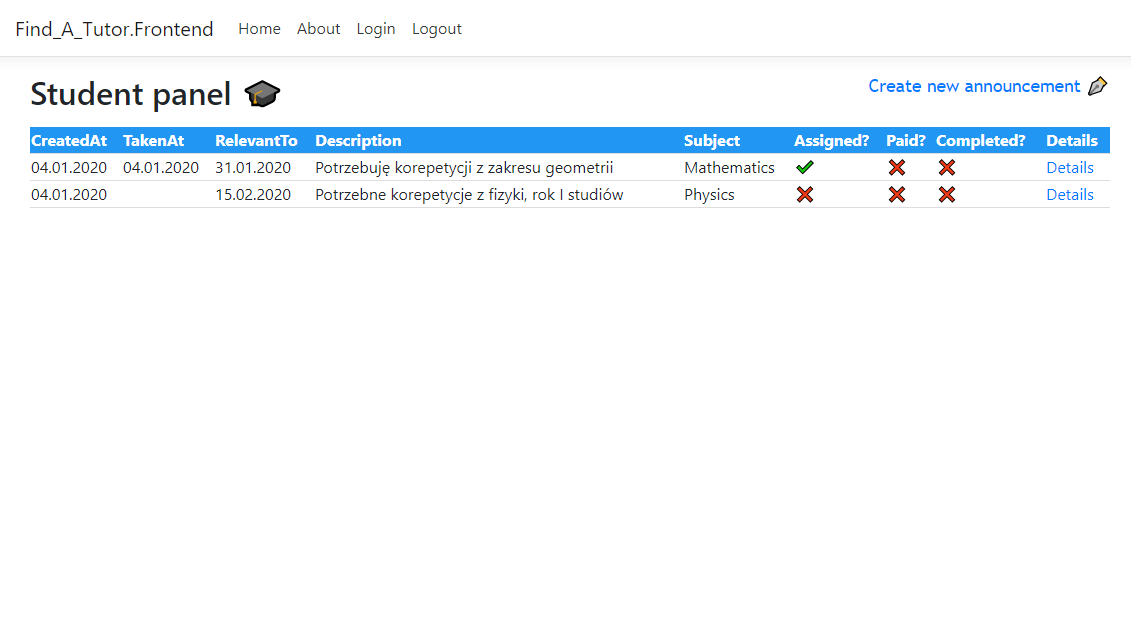
\includegraphics[width=1\textwidth]{images/chapter_4/student-assigned.png}
    \caption{Panel ucznia}
    \label{fig:student-assigned}
\end{figure}

Link "Details" przekierowuje użytkownika do szczegółów ogłoszenia, wraz z możliwością zapłacenia (Rysunek \ref{fig:details}). 
\begin{figure}[!htbp] 
    \centering
    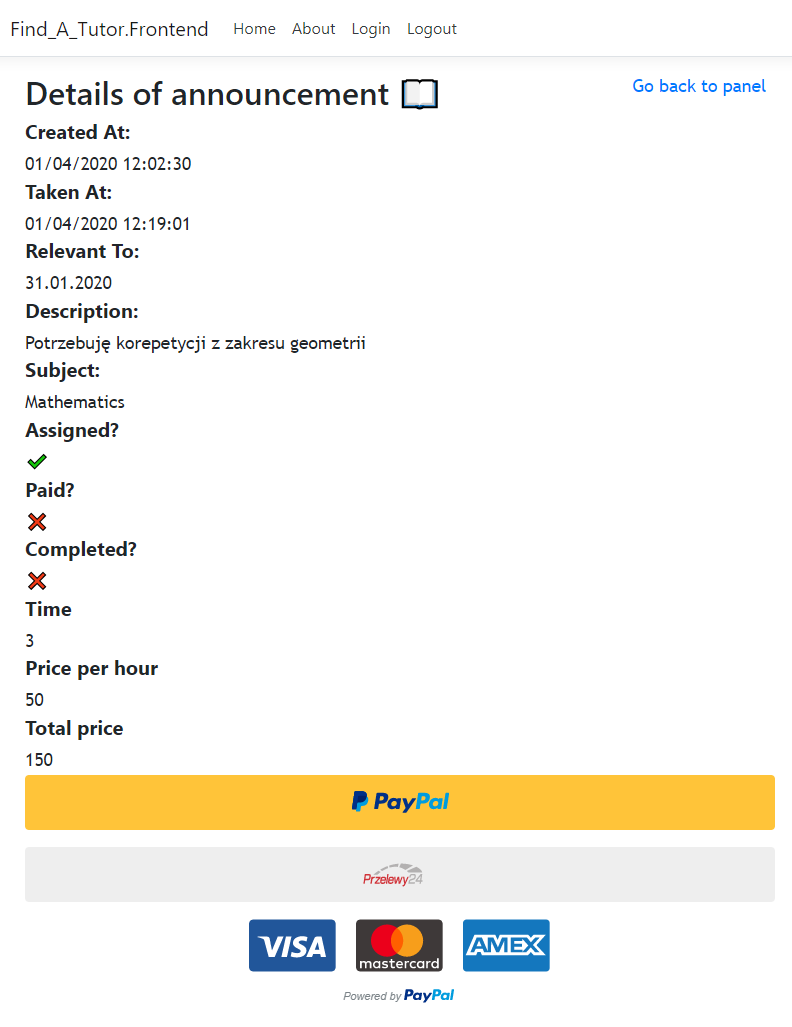
\includegraphics[width=1\textwidth]{images/chapter_4/details.png}
    \caption{Szczegóły ogłoszenia}
    \label{fig:details}
\end{figure}

"Total price" jest wynikiem mnożenia "Time" i "Price per hour". W celu zapłacenia, użytkownik wybiera sposób płatności, np. portfelem elektronicznym PayPal.

\begin{figure}[h]
    \centering
    \begin{subfigure}{.5\textwidth}
      \centering
      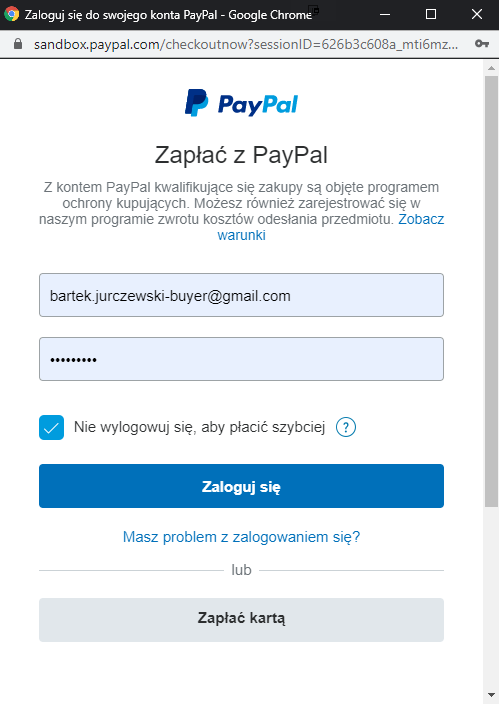
\includegraphics[width=.9\linewidth]{images/chapter_4/pay1.png}
      \caption{Logowanie do serwisu PayPal}
      \label{fig:paypal1}
    \end{subfigure}%
    \begin{subfigure}{.5\textwidth}
      \centering
      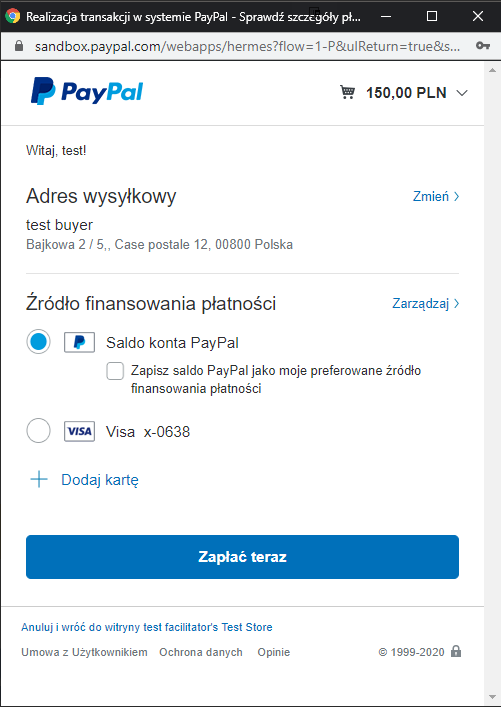
\includegraphics[width=.9\linewidth]{images/chapter_4/pay2.png}
      \caption{Potwierdzenie szczegółów płatności}
      \label{fig:paypal2}
    \end{subfigure}
    \caption{Płatność PayPalem}
    \label{fig:paypal}
\end{figure}

Dokonanie płatności zostało pokazane na rysunku \ref{fig:paypal}.

Po zapłaceniu, status ogłoszenia zostaje zaktualizowany. Został on pokazany na rysunku \ref{fig:details-paid}.
\begin{figure}[!htbp] 
    \centering
    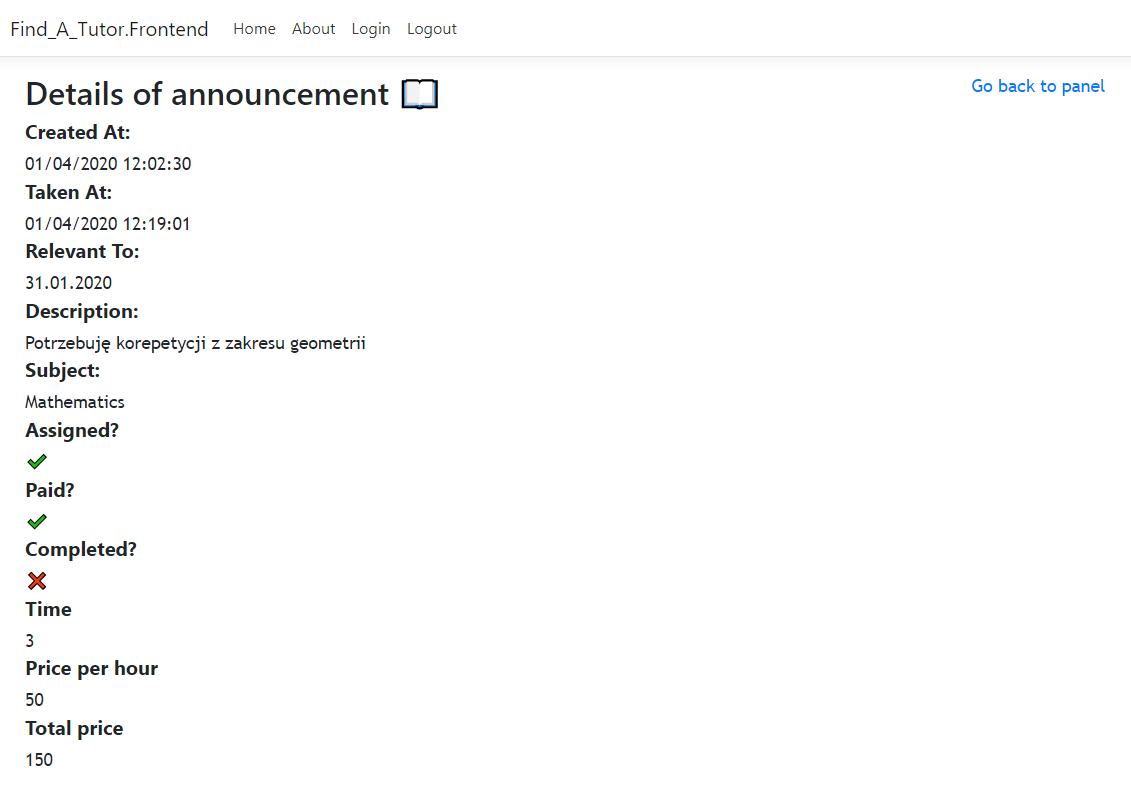
\includegraphics[width=1\textwidth]{images/chapter_4/details-paid.png}
    \caption{Szczegóły ogłoszenia po zapłaceniu}
    \label{fig:details-paid}
\end{figure}

\subsection{Wylogowanie}
Po naciśnięciu przycisku "Logout", na każdej z podstron, następuję zamknięcie sesji i wylogowanie z aplikacji. \newline

\textit{Aplikacja Find-A-Tutor zapewnia wszystkie potrzebne funkcjonalności dostarczając łatwy w obsłudze i wygodny portal do obsługi korepetycji.}

%%%%%%%%%%%%%%%%%%%%%%%%%%%%%%%%%%%%%%%%%%%%%%%%%%%%%%%%%%%%
%% Wnioski
%%%%%%%%%%%%%%%%%%%%%%%%%%%%%%%%%%%%%%%%%%%%%%%%%%%%%%%%%%%%
\section{Podsumowanie}
Pierwszym etapem pracy była analiza dwóch rynków: usług i płatności internetowych. Analiza rynku usług dowiodła że dostępne rozwiązania, takie jak \url{www.olx.pl}, oferują tylko podstawowe funkcjonalności. Przede wszystkim brakuje w nich płatność cyfrowych (w jakiekolwiek formie). Dodatkowo pomogła ona dostrzec nisze - rynek korepetycji, który mimo podstawowego zagospodarowania, popełnia błędy całego rynku usług. W dalszej części pracy została dokonana analiza rynku płatności cyfrowych w celu dostarczenia jak najlepszego systemu dla użytkownika końcowego. W analizie zostały nie tylko porównane obecne rozwiązania (przelewy tradycyjne, pay-by-link, karta płatnicza i portfele elektroniczne), ale także spośród zwycięzcy na tym polu - portfeli elektronicznych - zostało przeprowadzone zestawienie obecnych liderów na tym rynku. Zwycięskim rozwiązaniem okazał się PayPal. 

Bezpośrednim celem pracy było dostarczenie aplikacji webowej która w łatwy sposób pozwoli na zarządzanie korepetycjami ze strony ucznia jak i nauczyciela. Rozwiązanie takie zostało wykonane w sposób modularny, zgodnie z \textit{Czystą Architekturą}. Aplikacja ta jest otwarta na modyfikację w przyszłości, jak i na wymianę poszczególnych elementów. Ponadto, struktura aplikacji pozwoli w przyszłości zastosować implementację innych systemów płatności. Rzutuje to przede wszystkim na cykl życia aplikacji, która przez kolejne lata może nie być dalej rozwijana, ale same płatności portfelem elektronicznym będą aktualizowane. Od strony frontendowej, oferuje przejrzysty i czytelny interfejs który ułatwi użytkowanie tego portalu. 

Zaimplementowany system PayPal, który zwyciężył w analizie rynkowej, jest liderem płatności online. Inne firmy technologiczne, nawet te największe, takie jak Facebook czy Google są ze swoimi rozwiązaniami daleko za PayPalem. Pomimo tego że implementacja i testy nowych portfeli elektronicznych mogą być gotowe w niedalekiej przyszłości to dogonienie konkurencji pod względem przekonania do siebie użytkowników i utwierdzenie ich w rewolucyjności ich rozwiązania może zająć lata.

W przyszłości rynek usług będzie z pewnością ewoluował wchłaniając kolejne gałęzie przemysłu. Będzie to oznaczało zwiększenie agregatów ogłoszeń (np. \url{www.olx.pl}) jak i powstanie zupełnie nowych aplikacji takich jak \textit{Find-A-Tutor}. Udostępniona aplikacja może stanowić ciekawe rozwiązanie dla osób próbujących stworzyć autorską implemenetacje.

    \clearpage

%%%%%%%%%%%%%%%%%%%%%%%%%%%%%%%%%%%%%%%%%%%%%%%%%%%%%%%%%%%%
%% Indeks rysunków
%%%%%%%%%%%%%%%%%%%%%%%%%%%%%%%%%%%%%%%%%%%%%%%%%%%%%%%%%%%%     
    \section{Indeks rysunków}
        \listoffigures
    \clearpage    
    
%%%%%%%%%%%%%%%%%%%%%%%%%%%%%%%%%%%%%%%%%%%%%%%%%%%%%%%%%%%%
%% Indeks tabel
%%%%%%%%%%%%%%%%%%%%%%%%%%%%%%%%%%%%%%%%%%%%%%%%%%%%%%%%%%%% 
    \section{Indeks tabel}
        \listoftables
    \clearpage
    
%%%%%%%%%%%%%%%%%%%%%%%%%%%%%%%%%%%%%%%%%%%%%%%%%%%%%%%%%%%%
%% Bibliografia
%%%%%%%%%%%%%%%%%%%%%%%%%%%%%%%%%%%%%%%%%%%%%%%%%%%%%%%%%%%%     
    \section{Bibliografia}
    \renewcommand{\section}[2]{}
    \begin{thebibliography}{99}
    
%%%%%%%%%%%%%%%%%%%%%%%%%%%%%%%%%%%%%%%%%%%%%%%%%%%%%%%%%%%%
%% Chapter 1
%%%%%%%%%%%%%%%%%%%%%%%%%%%%%%%%%%%%%%%%%%%%%%%%%%%%%%%%%%%% 
    \bibitem{internet-users} 
    World Internet Users and 2019 Population Stats
    \url{https://www.internetworldstats.com/stats.htm}, dostęp 24-11-2019

    \bibitem{computers} 
    Computers sold this year
    \url{https://www.worldometers.info/computers/}, dostęp 24-11-2019
     
    \bibitem{ranking} 
    Ranking sklepów internetowych 2019
    \url{http://static.opineo.pl/press/dl/ranking-sklepow-internetowych-opineo-2019.pdf}, dostęp 28-11-2019
    
%%%%%%%%%%%%%%%%%%%%%%%%%%%%%%%%%%%%%%%%%%%%%%%%%%%%%%%%%%%%
%% Chapter 2
%%%%%%%%%%%%%%%%%%%%%%%%%%%%%%%%%%%%%%%%%%%%%%%%%%%%%%%%%%%% 
    \bibitem{allegro-wywiad} 
    Bakker o Allegro.pl: Cel był jasny. W e-commerce mógł być tylko jeden gracz
    \url{https://polskatimes.pl/bakker-o-allegropl-cel-byl-jasny-w-ecommerce-mogl-byc-tylko-jeden-gracz/ar/664791}, dostęp 28-11-2019
    
    \bibitem{allegro-liczby} 
    Wyniki badania Gemius/PBI za lipiec 2017
    \url{https://www.gemius.pl/wydawcy-aktualnosci/wyniki-badania-gemiuspbi-za-lipiec-2017.html}, dostęp 28-11-2019
    
    \bibitem{olx-wywiad} 
    Meet OLX, the biggest Web company you’ve never heard of
    \url{https://fortune.com/2014/10/29/olx-emerging-markets/}, dostęp 28-11-2019
    
    \bibitem{olx-liczby} 
    Wyniki badania Gemius/PBI za styczeń 2019
    \url{https://www.gemius.pl/wszystkie-artykuly-aktualnosci/wyniki-badania-gemiuspbi-za-styczen-2019.html}, dostęp 28-11-2019
    
    \bibitem{gotowka} 
    Sondaż: Jak Polacy płacą w Internecie?
    \url{https://www.kir.pl/o-nas/aktualnosci/sondaz-jak-polacy-placa-w-internecie,142.html}, dostęp 30-11-2019
    
    \bibitem{backswap} 
    Klienci PKO BP, BZ WBK, mBanku, ING i Pekao na celowniku nowego malware
    \url{https://zaufanatrzeciastrona.pl/post/klienci-pko-bp-bz-wbk-mbanku-ing-i-pekao-na-celowniku-nowego-malware/}, dostęp 30-11-2019
    
    \bibitem{jak-placa-polacy} 
    Jak Polacy kupują i płacą przez internet? Co lubią, czego się boją?
    \url{https://www.shoper.pl/blog/jak-polacy-kupuja-i-placa-przez-internet/}, dostęp 1-12-2019
    
    \bibitem{chargeback} 
    Płatność kartą przez Internet
    \url{https://www.najlepszekonto.pl/platnosc-karta-przez-internet}, dostęp 2-12-2019
    
%%%%%%%%%%%%%%%%%%%%%%%%%%%%%%%%%%%%%%%%%%%%%%%%%%%%%%%%%%%%
%% Chapter 3
%%%%%%%%%%%%%%%%%%%%%%%%%%%%%%%%%%%%%%%%%%%%%%%%%%%%%%%%%%%% 
    \bibitem{funkcjonalne} 
    Wymagania funkcjonalne aplikacji internetowej
    \url{http://www.commint.pl/baza/wymagania-funkcjonalne-aplikacji-internetowej}, dostęp 10-12-2019
    
    \bibitem{niefunkcjonalne} 
    Wymagania niefunkcjonalne aplikacji internetowej
    \url{http://www.commint.pl/baza/wymagania-niefunkcjonalne-aplikacji-internetowej}, dostęp 10-12-2019
    
    \bibitem{chrome} 
    Browser Market Share Poland
    \url{https://gs.statcounter.com/browser-market-share/all/poland}, dostęp 10-12-2019
    
    \bibitem{clean-architecture} 
    Clean Architecture with ASP.NET Core 2.2
    \url{https://github.com/JasonGT/NorthwindTraders/blob/master/Docs/Slides.pdf}, dostęp 19-12-2019
    \url{https://www.youtube.com/watch?v=_lwCVE_XgqI}, dostęp 20-12-2019
    
    \bibitem{dotnet-core} 
    Wprowadzenie do platformy ASP.NET Core
    \url{https://docs.microsoft.com/pl-pl/aspnet/core/?view=aspnetcore-2.1}, dostęp 21-12-2019
    
    \bibitem{csharp} 
    Wprowadzenie do języka \Csharp i systemu .NET Framework
    \url{https://docs.microsoft.com/pl-pl/dotnet/csharp/getting-started/introduction-to-the-csharp-language-and-the-net-framework}, dostęp 21-12-2019
    
    \bibitem{health-checks} 
    Health checks in ASP.NET Core
    \url{https://docs.microsoft.com/en-gb/aspnet/core/host-and-deploy/health-checks?view=aspnetcore-3.1}, dostęp 21-12-2019
    
    \bibitem{health-checks-github} 
    AspNetCore.Diagnostics.HealthChecks
    \url{https://github.com/xabaril/AspNetCore.Diagnostics.HealthChecks}, dostęp 21-12-2019
    
    \bibitem{json} 
    Introducing JSON
    \url{https://www.json.org/json-en.html}, dostęp 21-12-2019
    
    \bibitem{sekurak-jwt} 
    (Nie) bezpieczeństwa JWT (JSON Web Token)
    \url{https://sekurak.pl/jwt-security-ebook.pdf}, dostęp 25-12-2019
    
    \bibitem{token-diagram} 
    JSON Web Tokens (JWT)
    \url{https://blog.i-systems.pl/json-web-tokens-jwt/}, dostęp 27-12-2019
    
    \bibitem{http} 
    Hypertext Transfer Protocol -- HTTP/1.1
    \url{https://www.ietf.org/rfc/rfc2616.txt}, dostęp 28-12-2019
    
    \bibitem{mvc} 
    ASP .Net MVC – pojęcia podstawowe
    \url{https://www.wojciechseweryn.pl/2018/07/07/asp-net-mvc-pojecia-podstawowe/}, dostęp 30-12-2019
    
    \bibitem{mvc-flow} 
    Paradygmat MVC Model-View-Controller
    \url{https://farmastron.pl/paradygmat-mvc-model-view-controller}, dostęp 30-12-2019
    
    \end{thebibliography}
\end{sloppypar}
\end{document}